\chapter{Benchmarking QUBO solvers}\label{benchmark}
This chapter first introduces related benchmarking work for QUBO problems and QUBO solvers. Then, we present our results for the solvers and datasets used for this study.

\section{Related benchmarking work}
One of the first benchmarking works for quantum annealing was conducted by Denchev et al. \yrcite{denchev2016computational}, who measured the performance of D-Wave quantum annealing on the older D-Wave 2X machine using specially crafted problems that have tall and narrow energy barriers separating local minima. Quantum annealing is expected to be $1.8 \times 10^8$ times faster than simulated annealing, which tends to fail with problems with such an energy landscape.


\outcite{b34} evaluated the performance of QAOA on the IBMQ backend and the D-Wave solver using instances of MaxCut and 2-satisfiability problems with up to 18 variables. The performance of the QAOA algorithm is inconsistent and underperforms quantum annealing in their problem set. More recently, \outcite{b35} also compared the performance of QAOA on the IBMQ backend and D-Wave quantum annealing on randomly generated Ising problems with cubic interaction terms and found that quantum annealing had superior performance over QAOA for all problem sizes.

\outcite{gomes2019classical} showed that the NNQS solving method with an RBM architecture produces good quality solutions for the max-cut problem with graph sizes of up to 256. \outcite{khandoker2023supplementing} uses recurrent neural networks as the NNQS architecture for the max-cut and travelling salesman problem and found that it outperforms SA. However, no direct study has compared performance across quantum annealing, QAOA, and NNQS.

\section{Results and Discussion}
Performance is shown for each dataset, accompanied by error bars representing each data point's unbiased standard error of the mean. Graphs with problem sizes on the x-axis are plotted with a log scale.

\subsection{NAE3SAT}

\begin{figure}[!htbp]
    \centering
    \subfloat[Normalized energy]{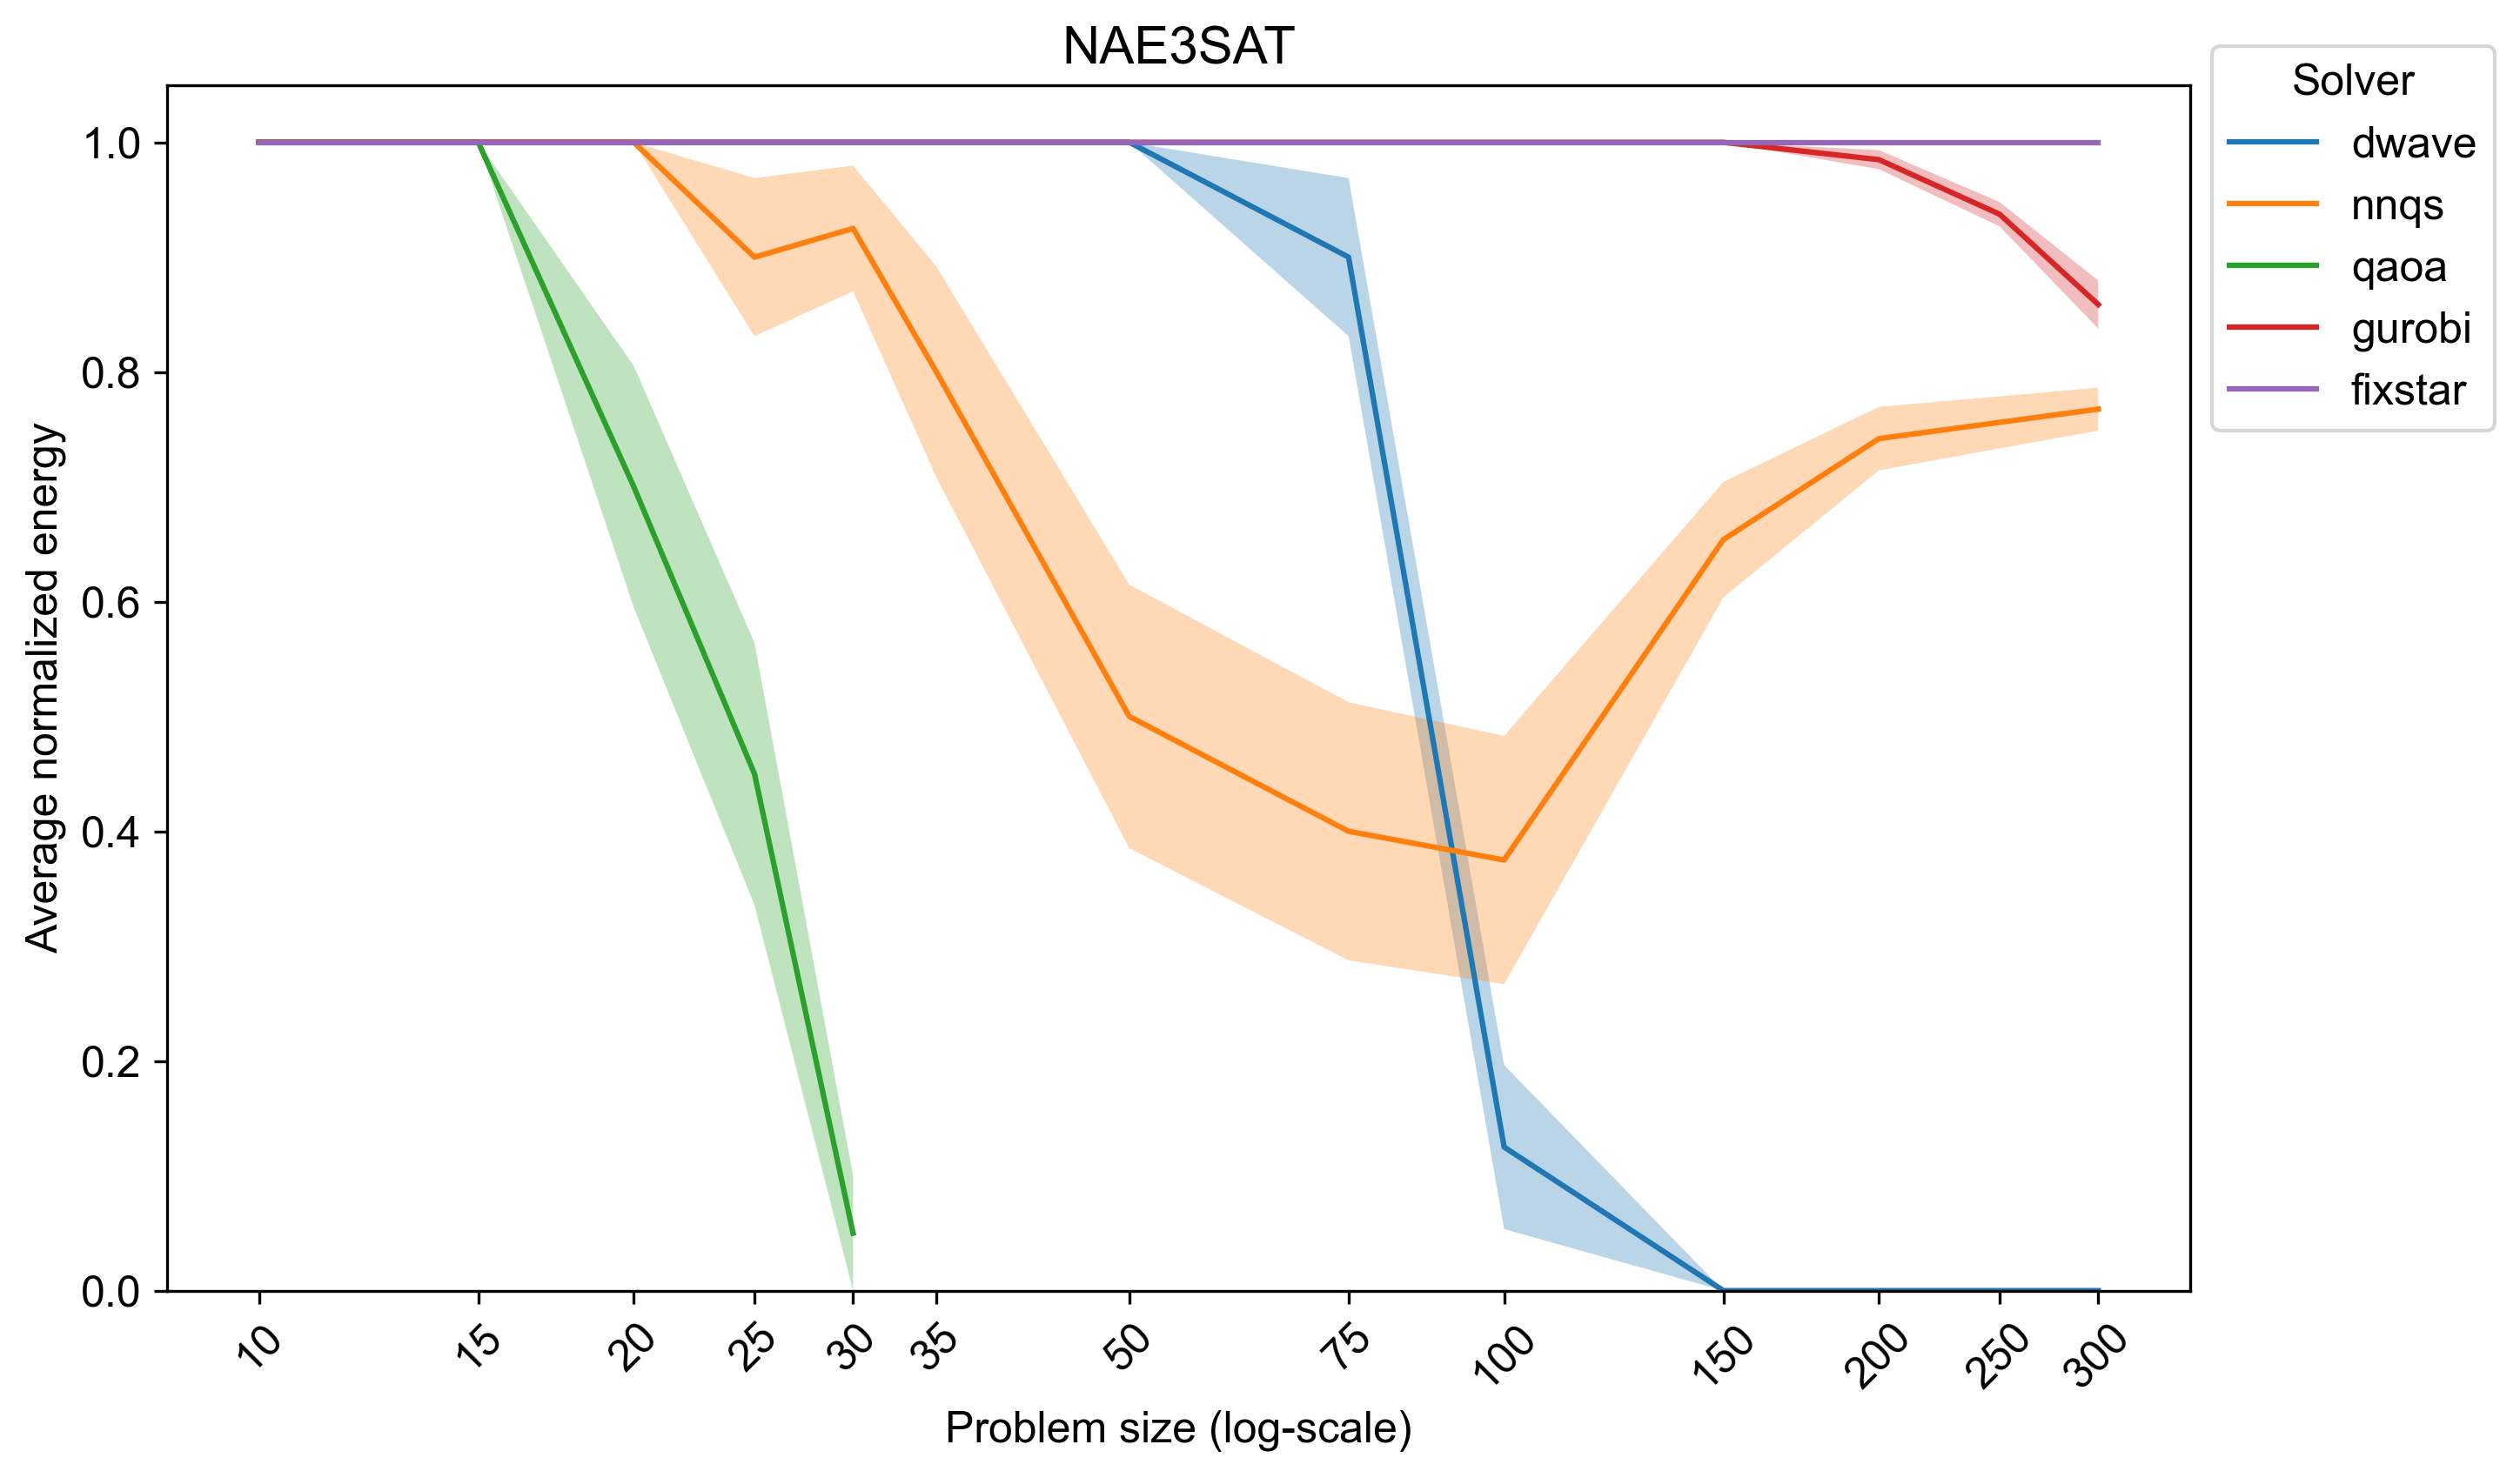
\includegraphics[width=0.9\textwidth]{images/nae3sat_all_size.png}}
    \\
    \subfloat[Success probability]{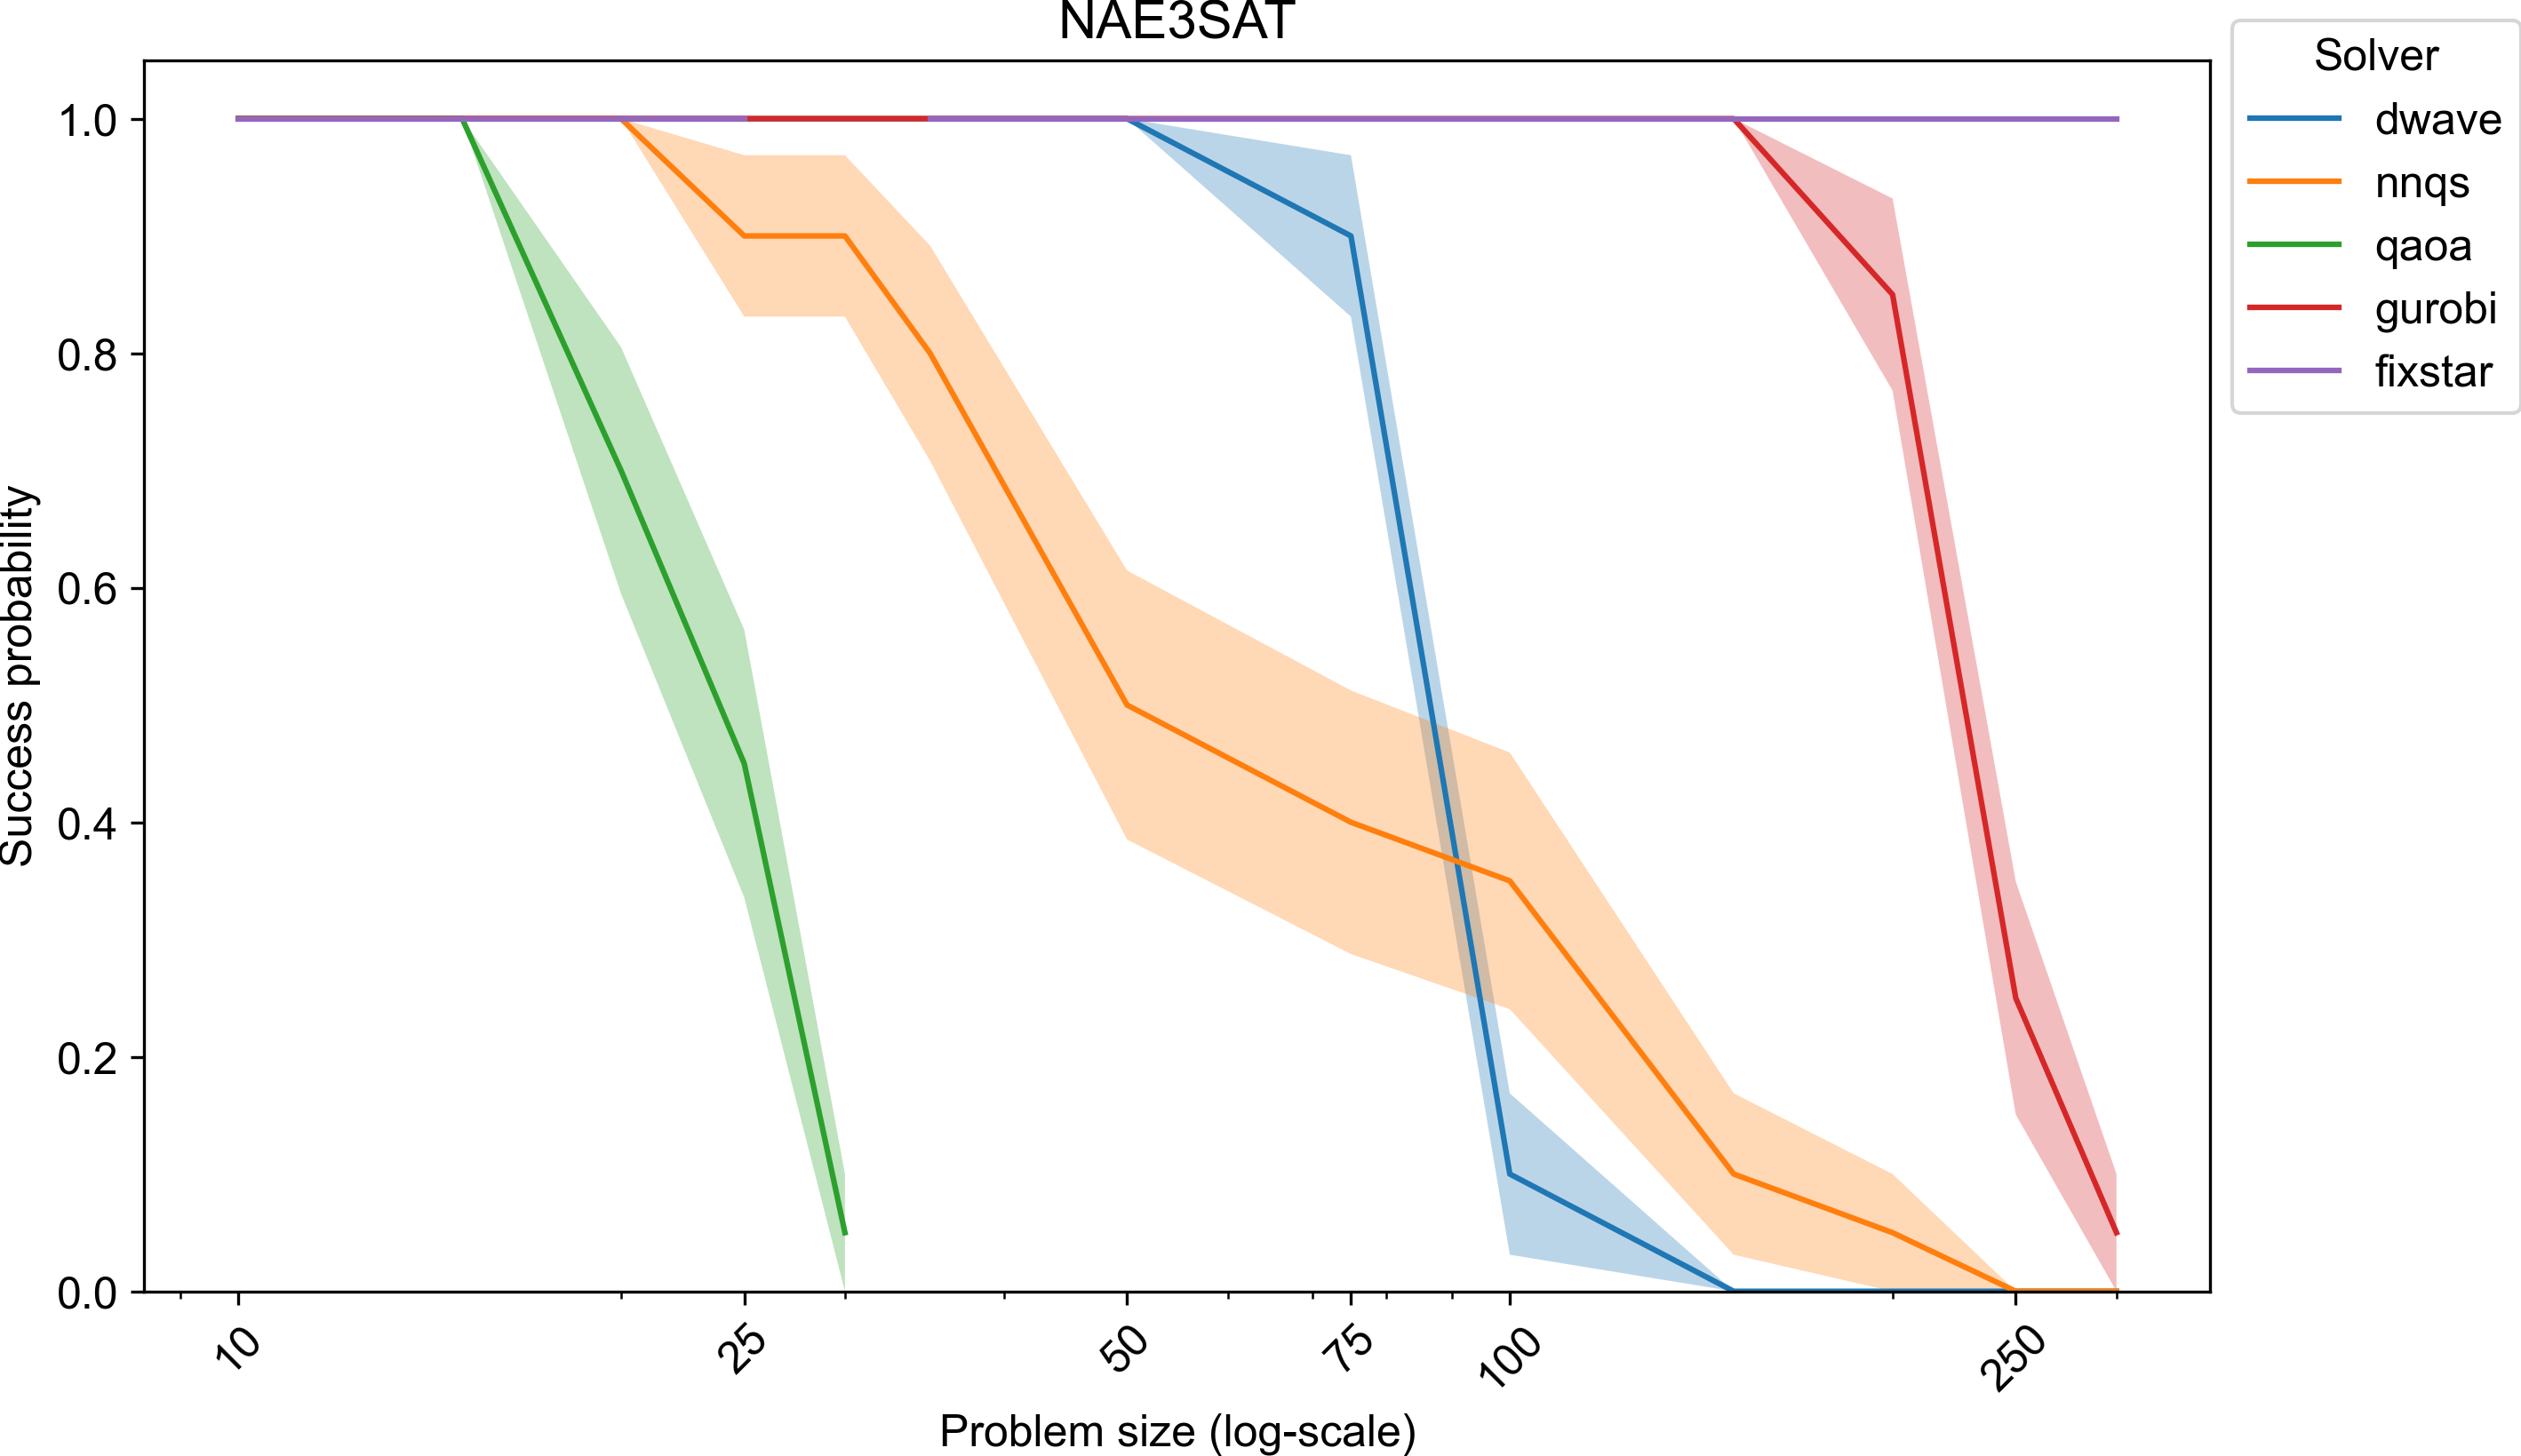
\includegraphics[width=0.9\textwidth]{images/nae3sat_all_success_size.png}}
    \caption{Performance of different solvers for NAE3SAT by problem size}
    \label{all-nae3sat-size}
\end{figure}

\begin{figure}[!htbp]
    \centering
    \subfloat[Normalized energy]{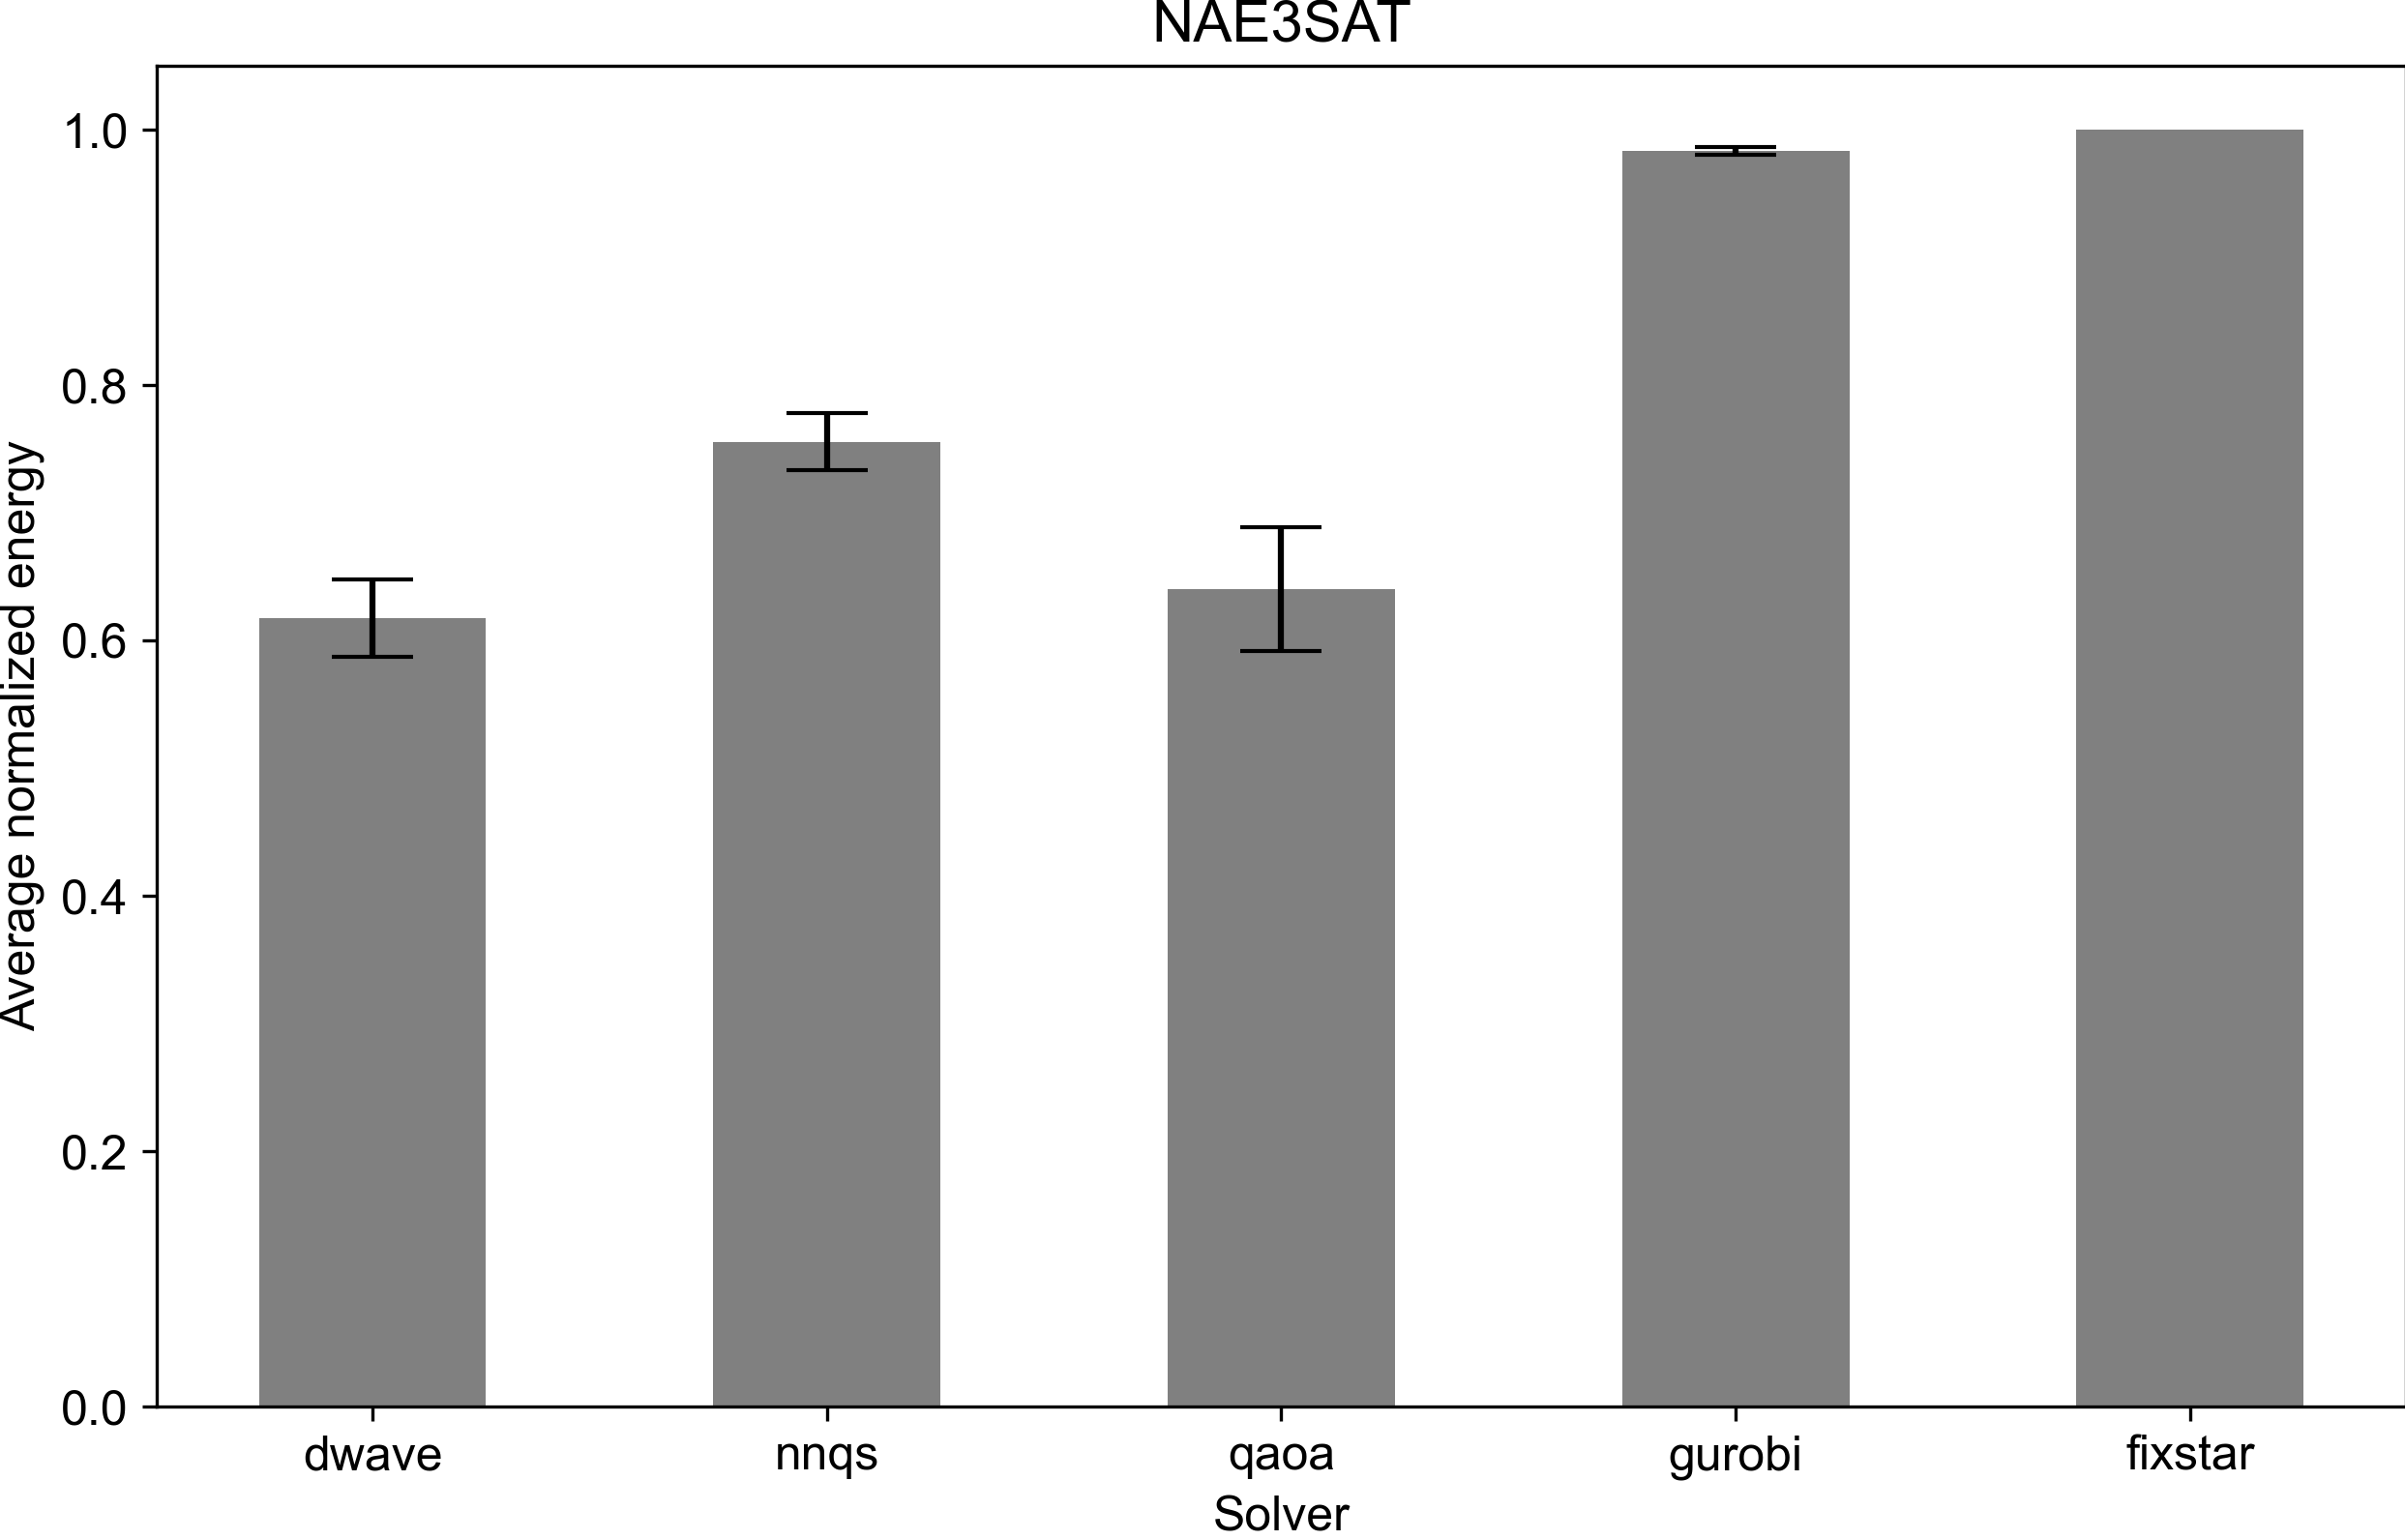
\includegraphics[width=0.49\textwidth]{images/nae3sat_all_avg.png}}\hfill
    \subfloat[Success probability]{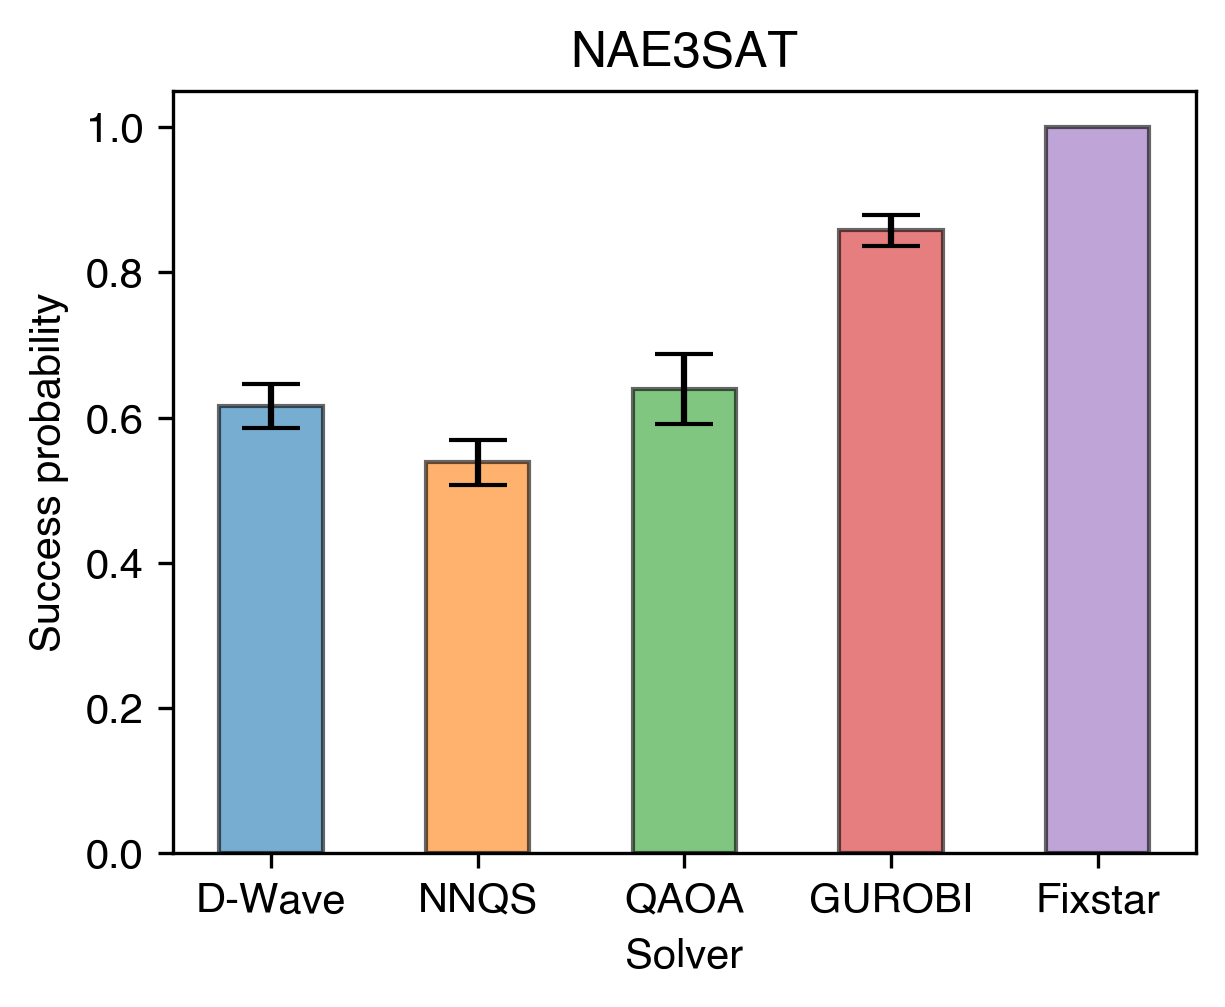
\includegraphics[width=0.49\textwidth]{images/nae3sat_all_success_avg.png}}
    \caption{Average performance of different solvers for NAE3SAT}
    \label{all-nae3sat-average}
\end{figure}

Performance by size for the NAE3SAT dataset in \autoref{all-nae3sat-size} and average performance is shown in \autoref{all-nae3sat-average}. The D-wave solver and NNQS could both solve problems up to $n=300$. However, multiple embedding requests were required for problems of size $300$ for the D-wave Pegasus topology, which suggests that $n=300$ might be near the D-wave size limit for the NAE3SAT problem. QAOA could only solve problems of up to $n=30$ due to the limitations on the number of qubits of the simulator.

In terms of performance, the D-wave solver performs well up to $n=50$ with a success probability of $1$. For larger problem sizes, the performance of the D-wave solver drops off sharply. The NNQS performs well up to $n=20$, with the success probability and normalised energy gradually decreasing until $n=300$. The QAOA solver performs well up to $n=15$, and performance decreases until $n=30$. Between the classical solvers, the Fixstars QUBO solver performs better than the GUROBI optimiser at larger problem sizes ($>150$). Both classical solvers outperform the quantum-inspired solvers.

Overall, the NNQS has the highest average normalised energy among the three quantum-inspired solvers but has the lowest success probability, which is likely due to it being able to solve problems of larger sizes that the D-wave Annealer and QAOA solver cannot handle. The QAOA solver has the highest success probability but can only handle problems up to $n=30$.

\subsection{Max-cut}

\begin{figure}[!htbp]
    \centering
    \subfloat[Normalized energy]{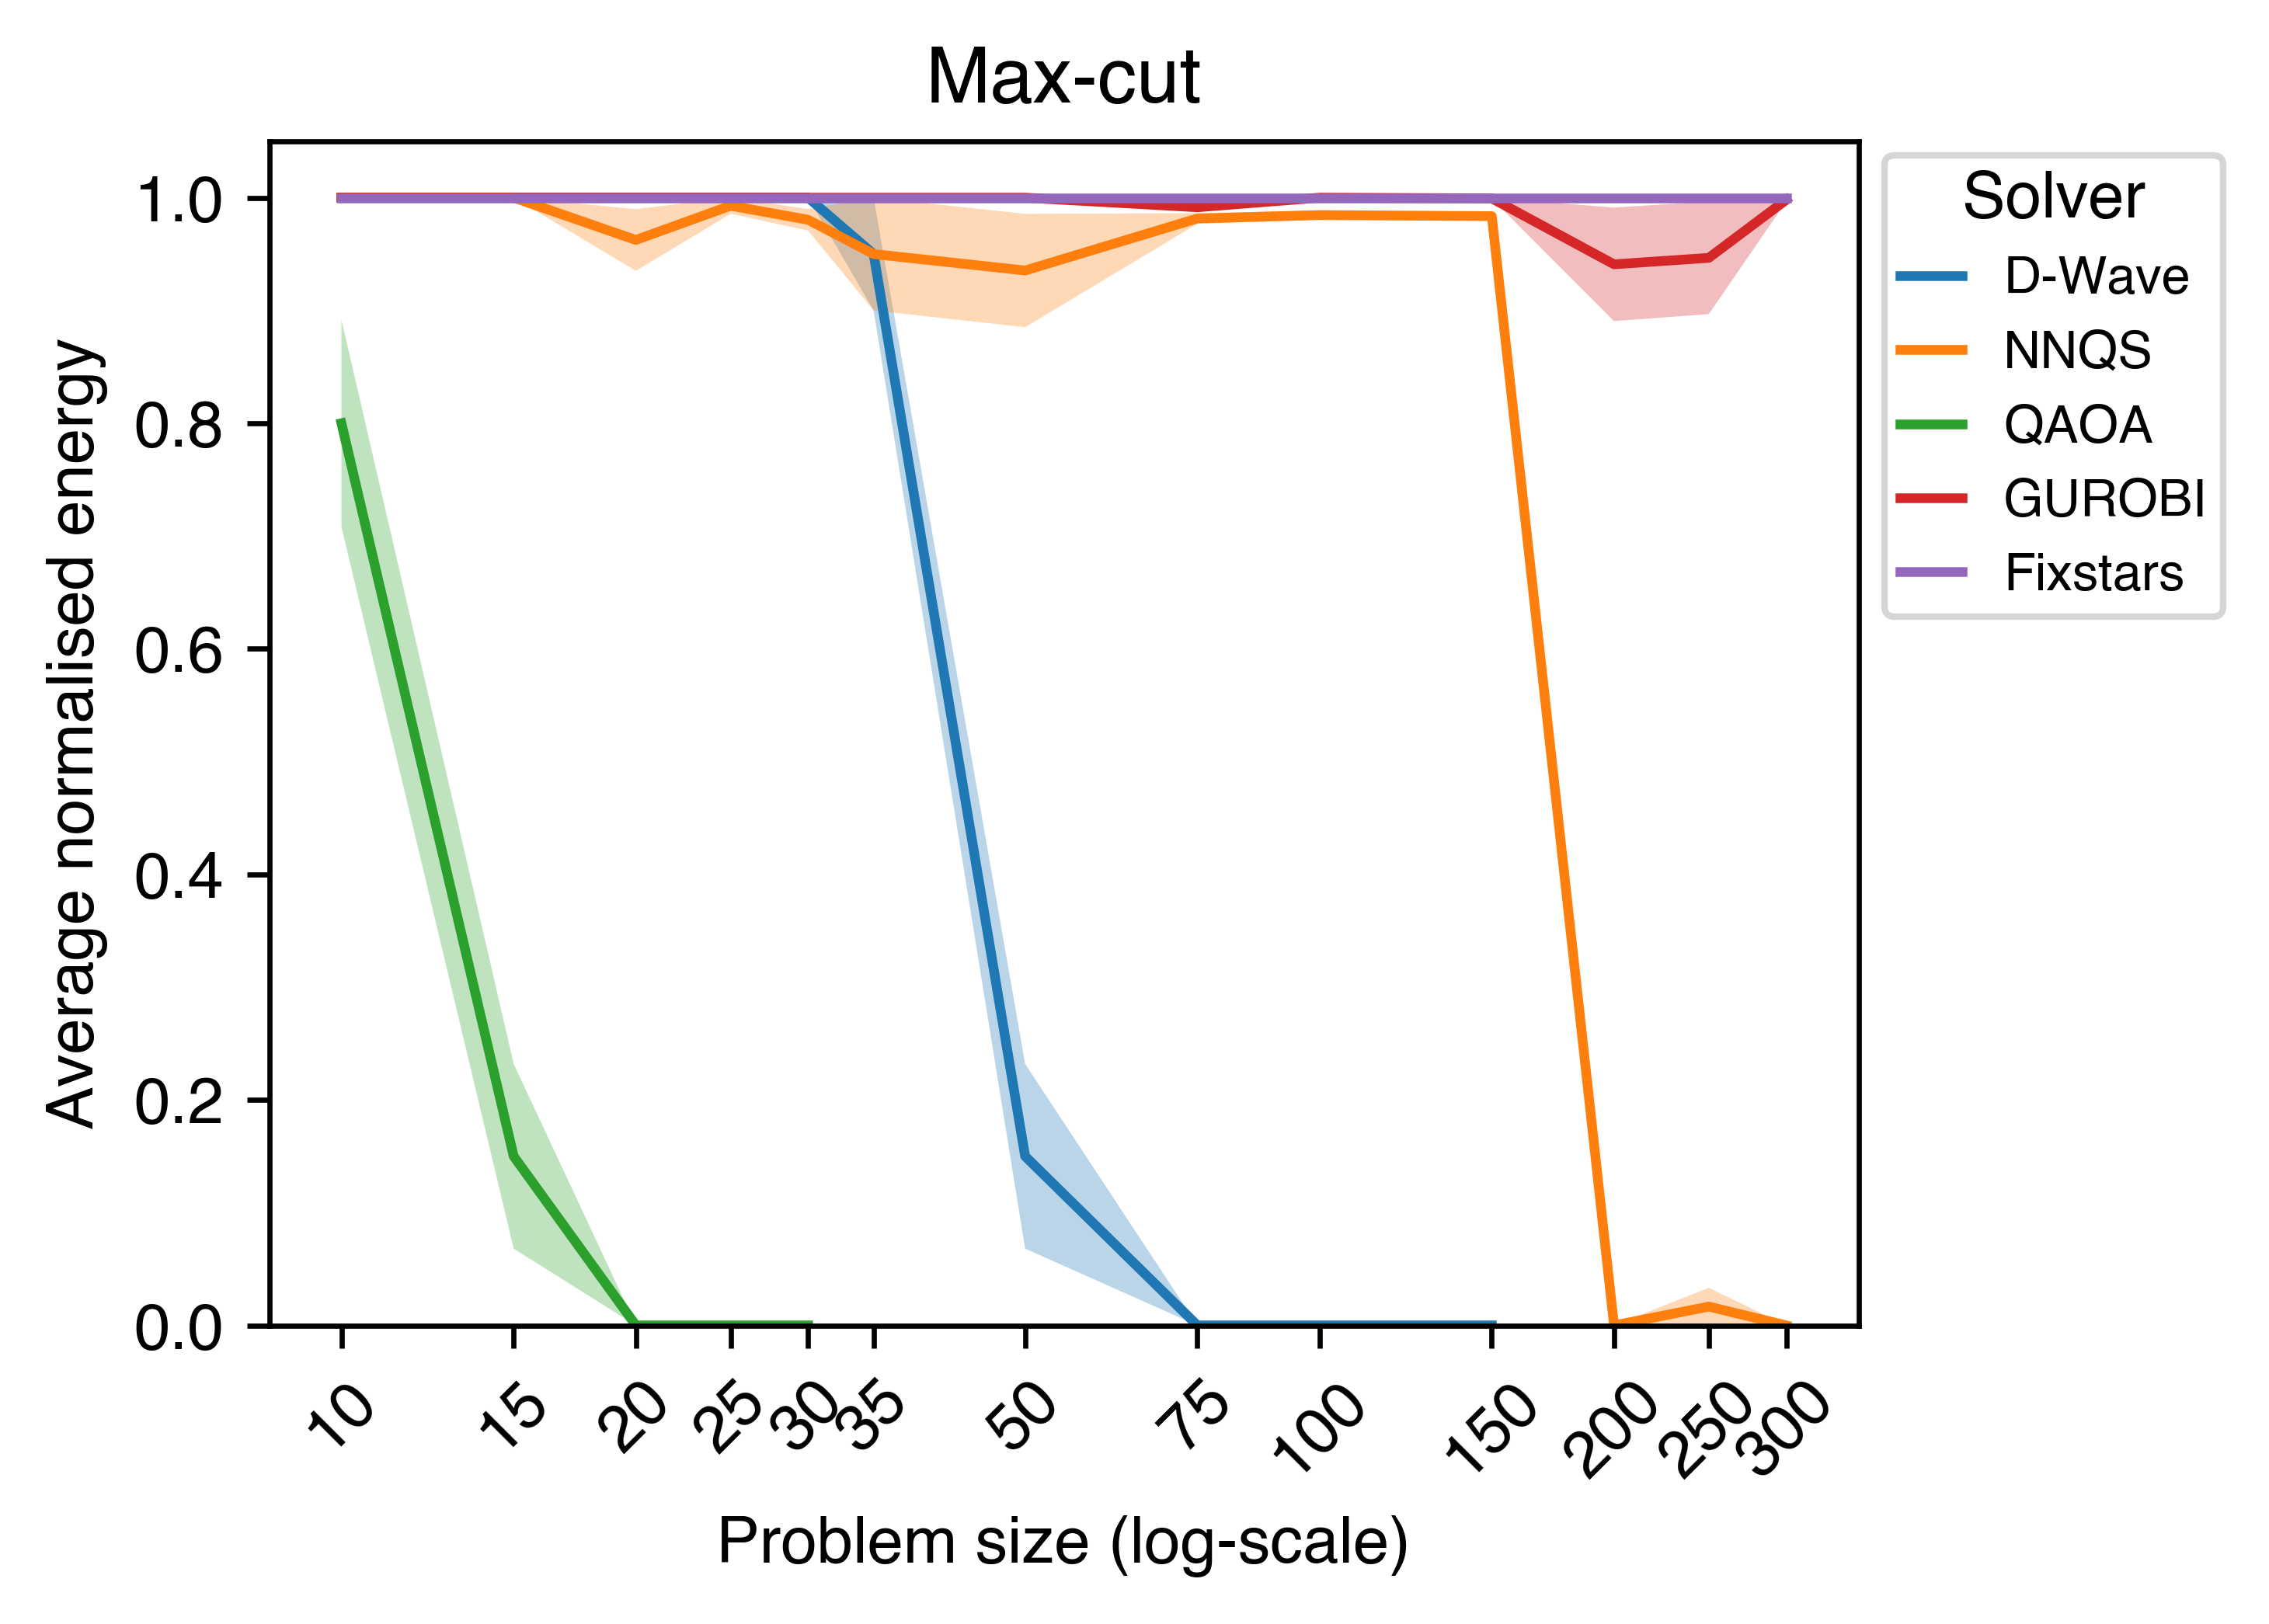
\includegraphics[width=0.9\textwidth]{images/maxcut_all_size.png}}
    \\
    \subfloat[Success probability]{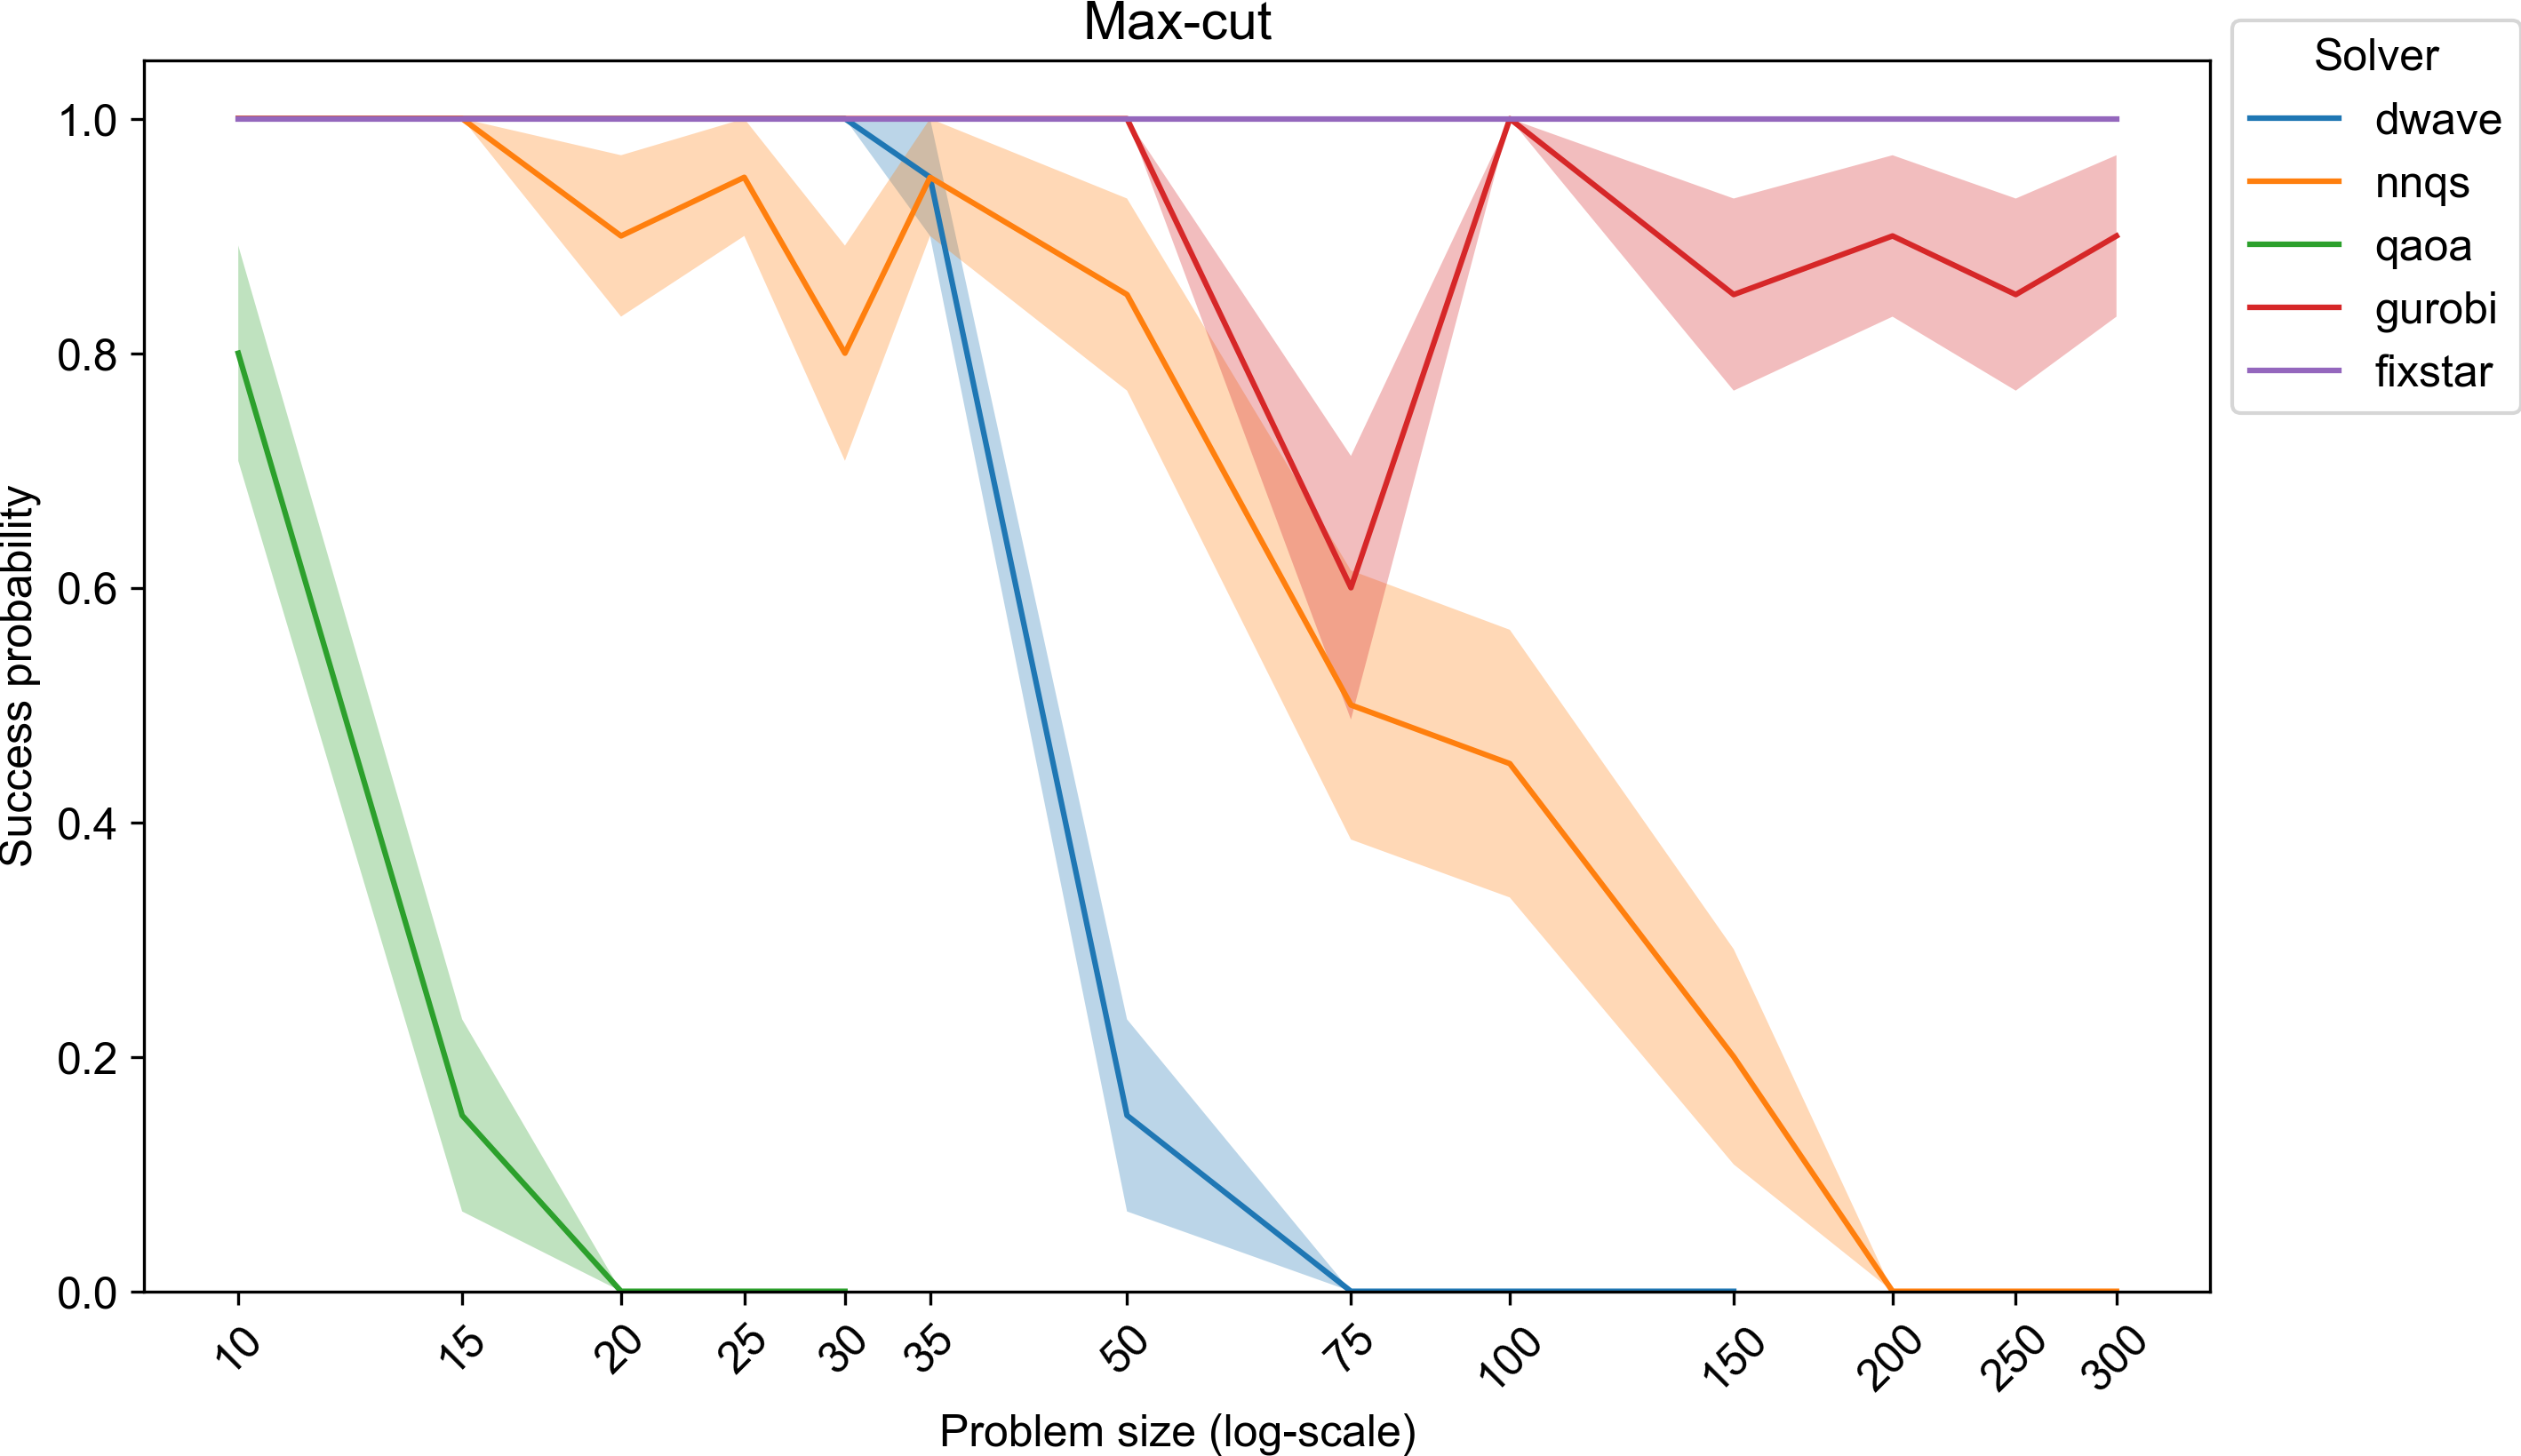
\includegraphics[width=0.9\textwidth]{images/maxcut_all_success_size.png}}
    \caption{Performance of different solvers for max-cut by problem size}
    \label{all-maxcut-size}
\end{figure}

\begin{figure}[!htbp]
    \centering
    \subfloat[Normalized energy]{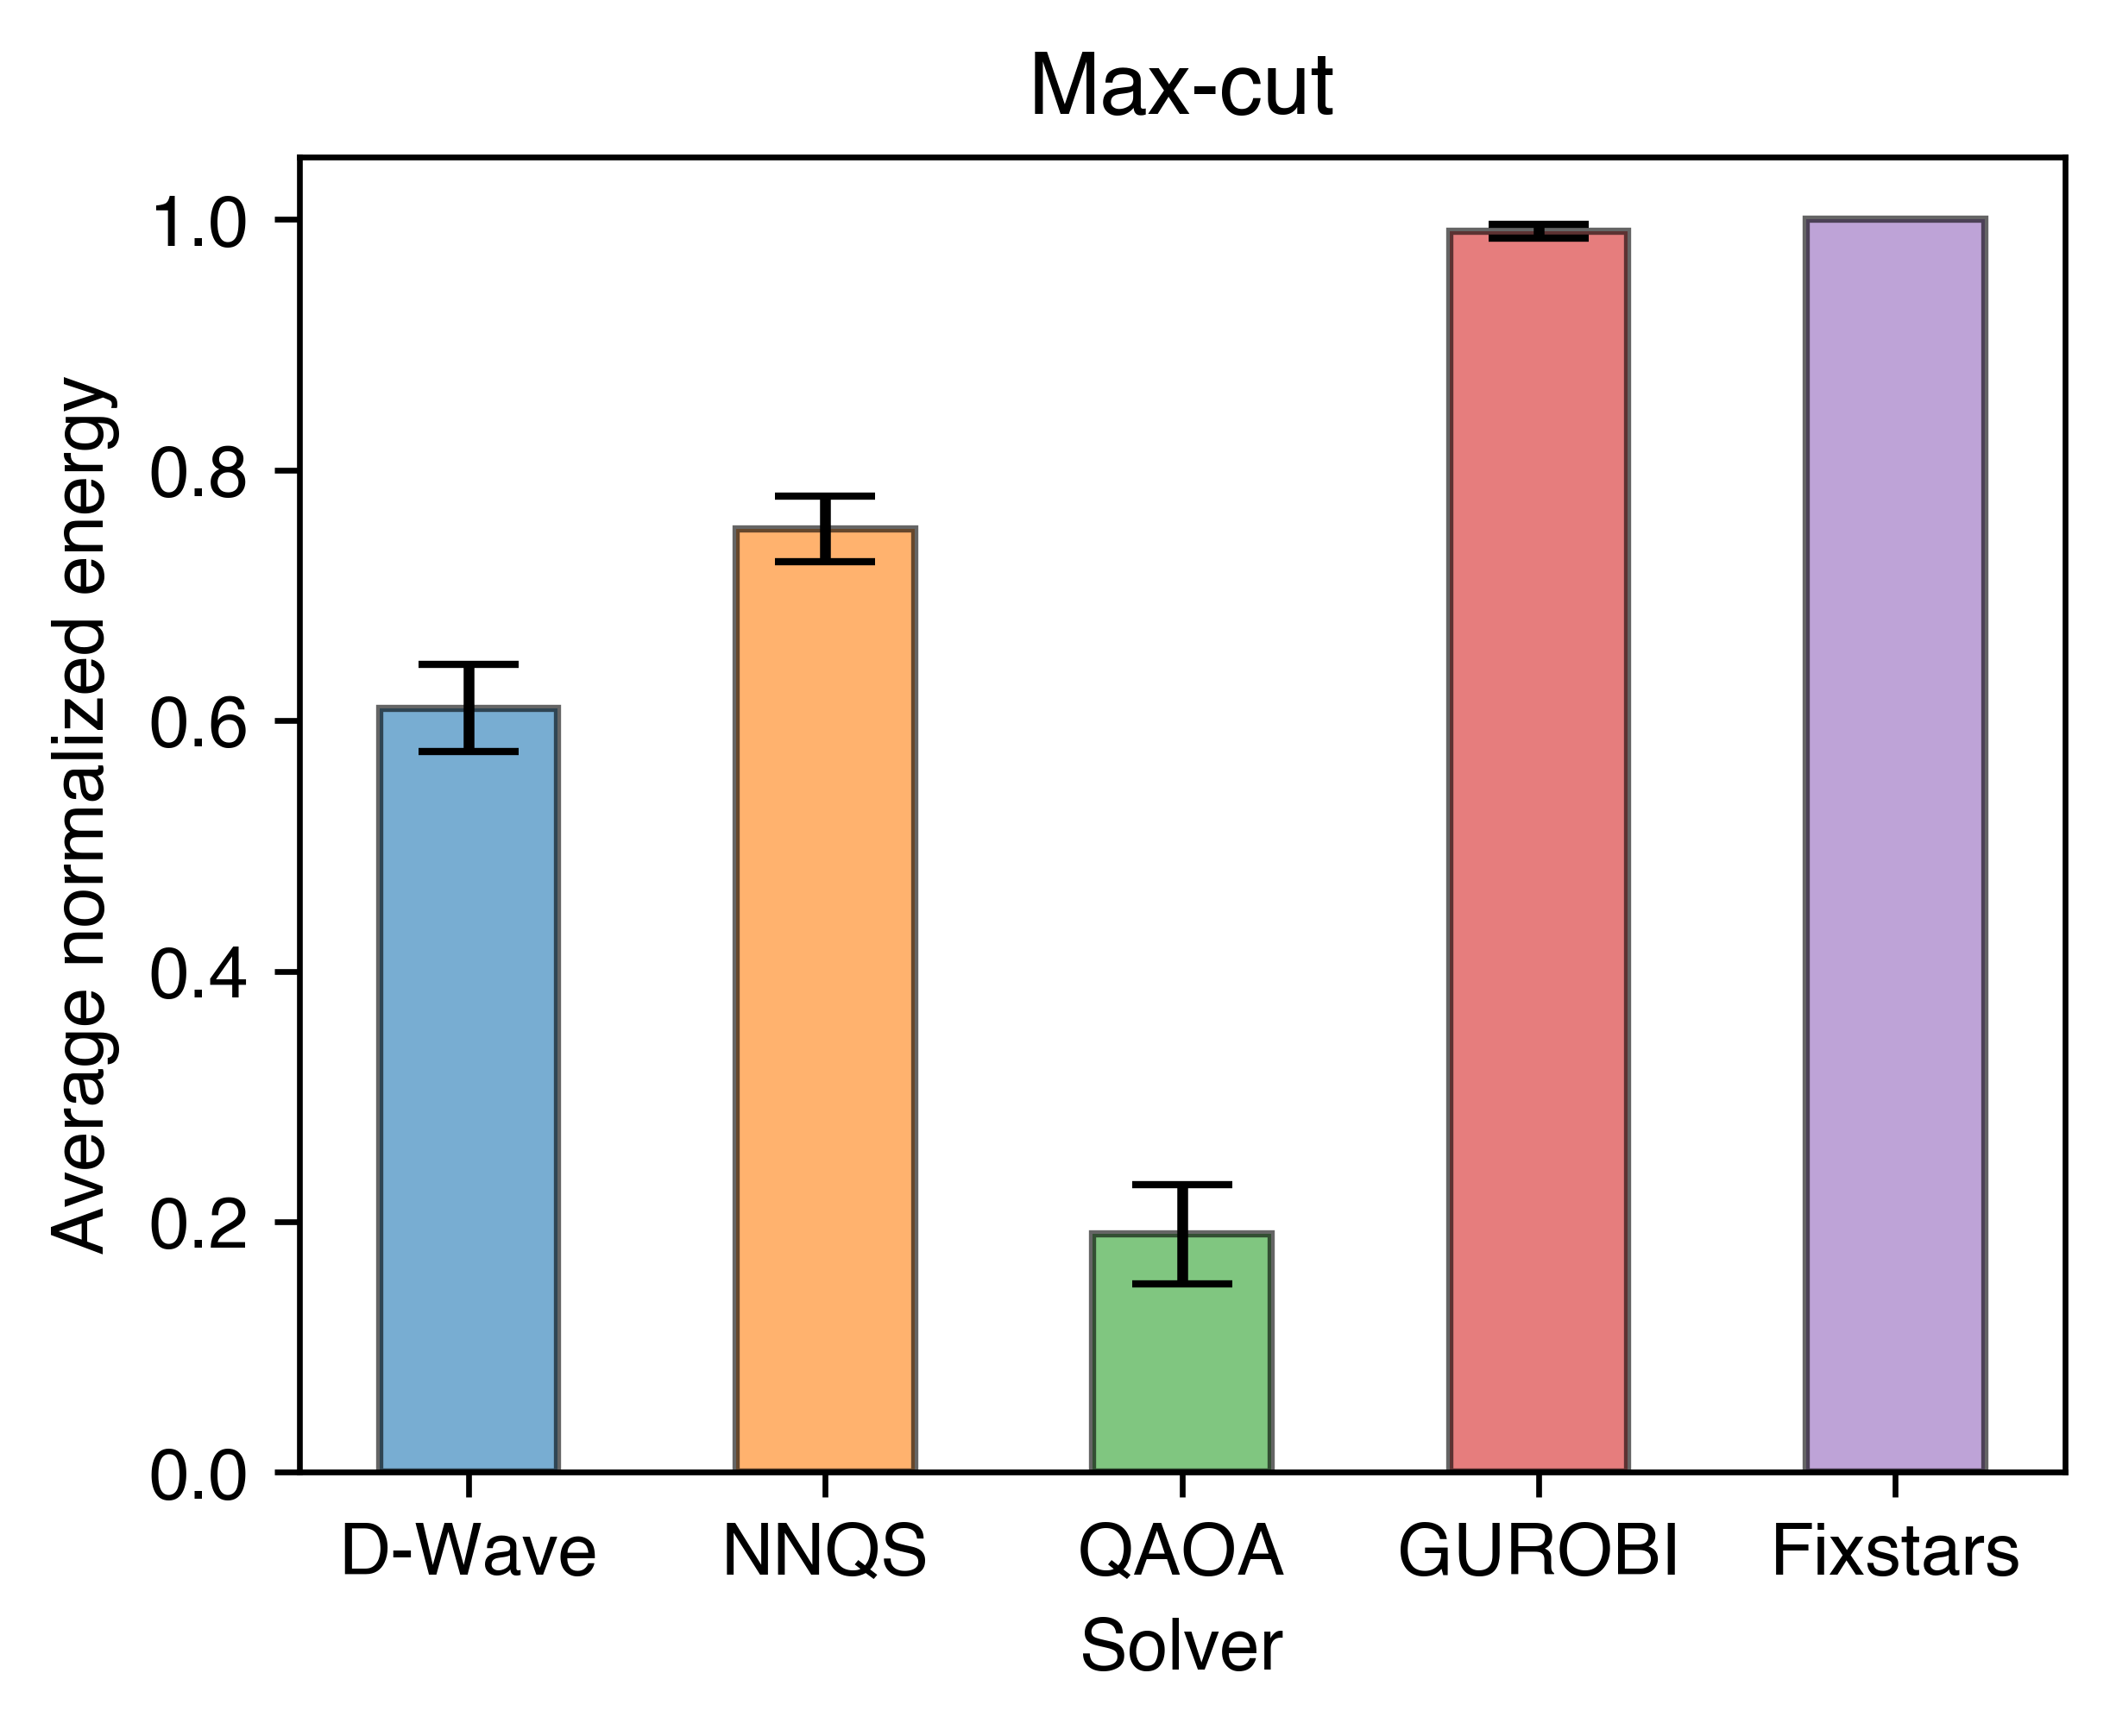
\includegraphics[width=0.49\textwidth]{images/maxcut_all_avg.png}}\hfill
    \subfloat[Success probability]{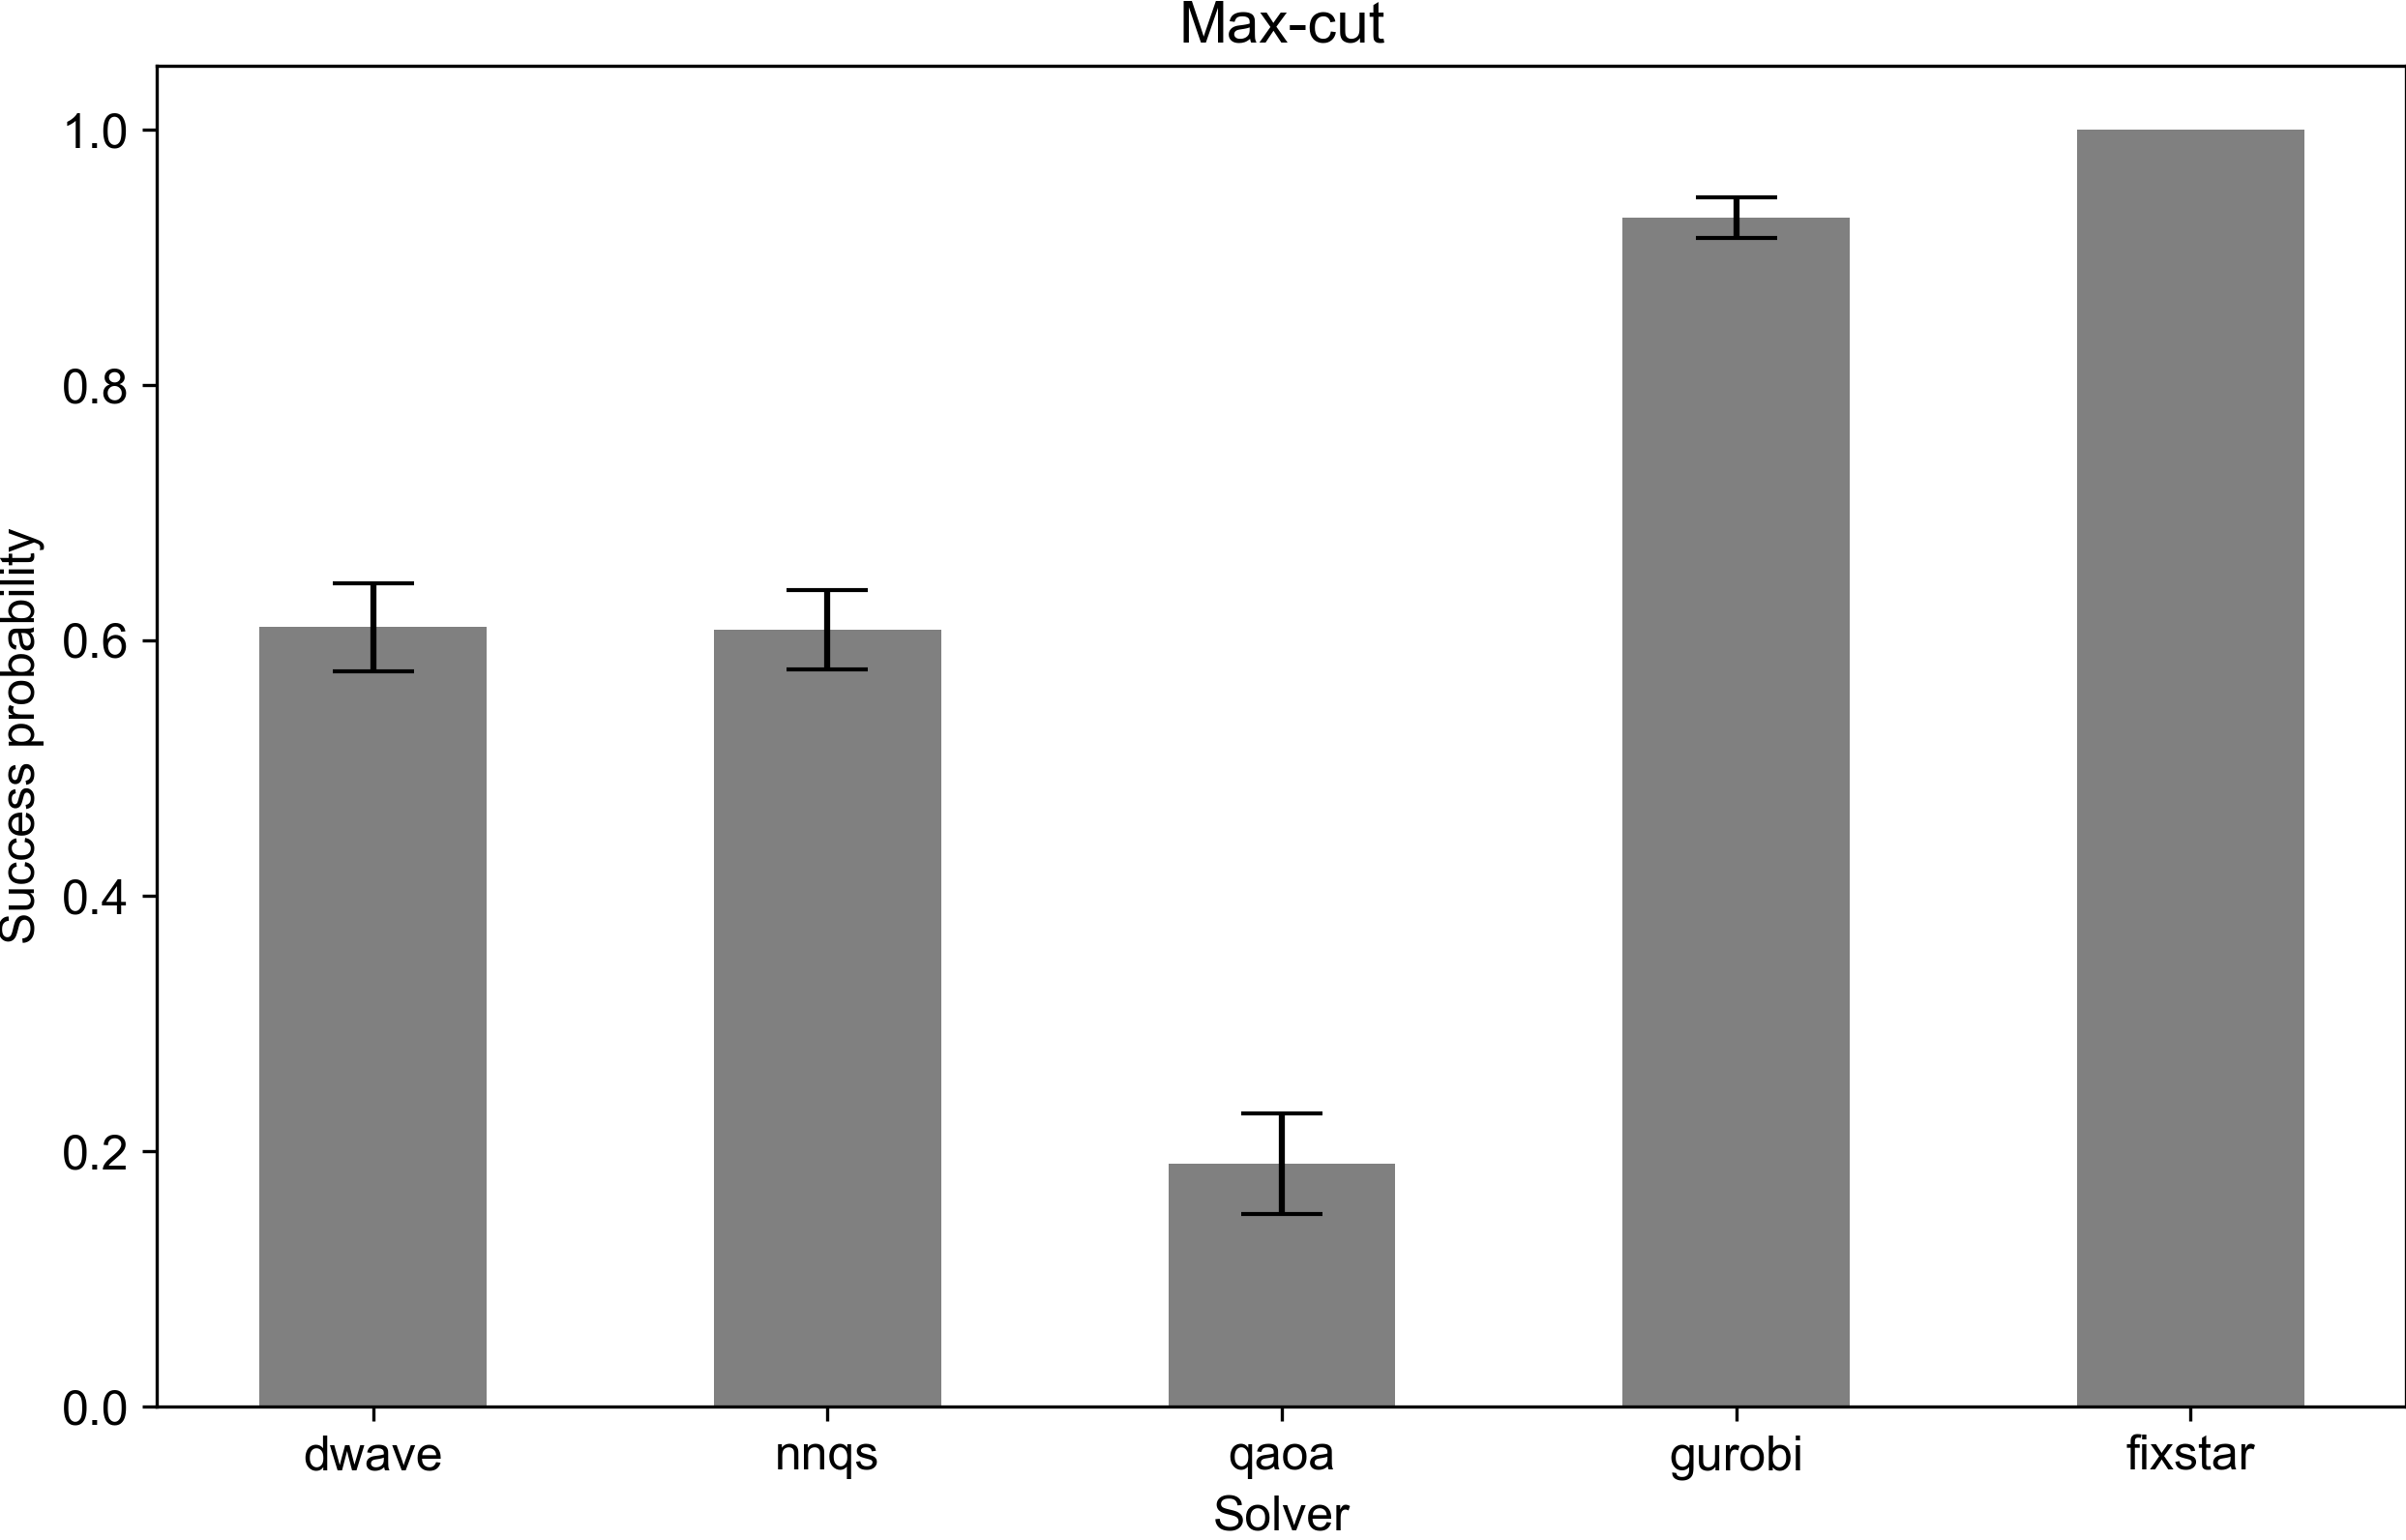
\includegraphics[width=0.49\textwidth]{images/maxcut_all_success_avg.png}}
    \caption{Average performance of different solvers for max-cut}
    \label{all-maxcut-average}
\end{figure}

Performance by size for the max-cut dataset is shown in \autoref{all-maxcut-size}, and average performance is shown in \autoref{all-maxcut-average}. For the max-cut problem, the D-wave solver could only handle problem sizes up to $n=150$ due to the need for minor embedding onto the pegasus topology. QAOA solved problems of up to $n=30$ due to the limitations of the simulator.

In terms of performance, the D-wave solver performs well up to $n=30$, and performance drops off sharply for larger problems. The NNQS performs well at $n=150$, although the success probability decreases for problem sizes over $50$. The QAOA solver performs well only for $n=10$, with performance decreasing for larger problems.

Overall, the NNQS has the highest average normalised energy among the three quantum-inspired solvers and has a slightly lower success probability than the D-wave solver. The QAOA solver performs poorly in both metrics.

\subsection{SK model}

\begin{figure}[!htbp]
    \centering
    \subfloat[Normalized energy]{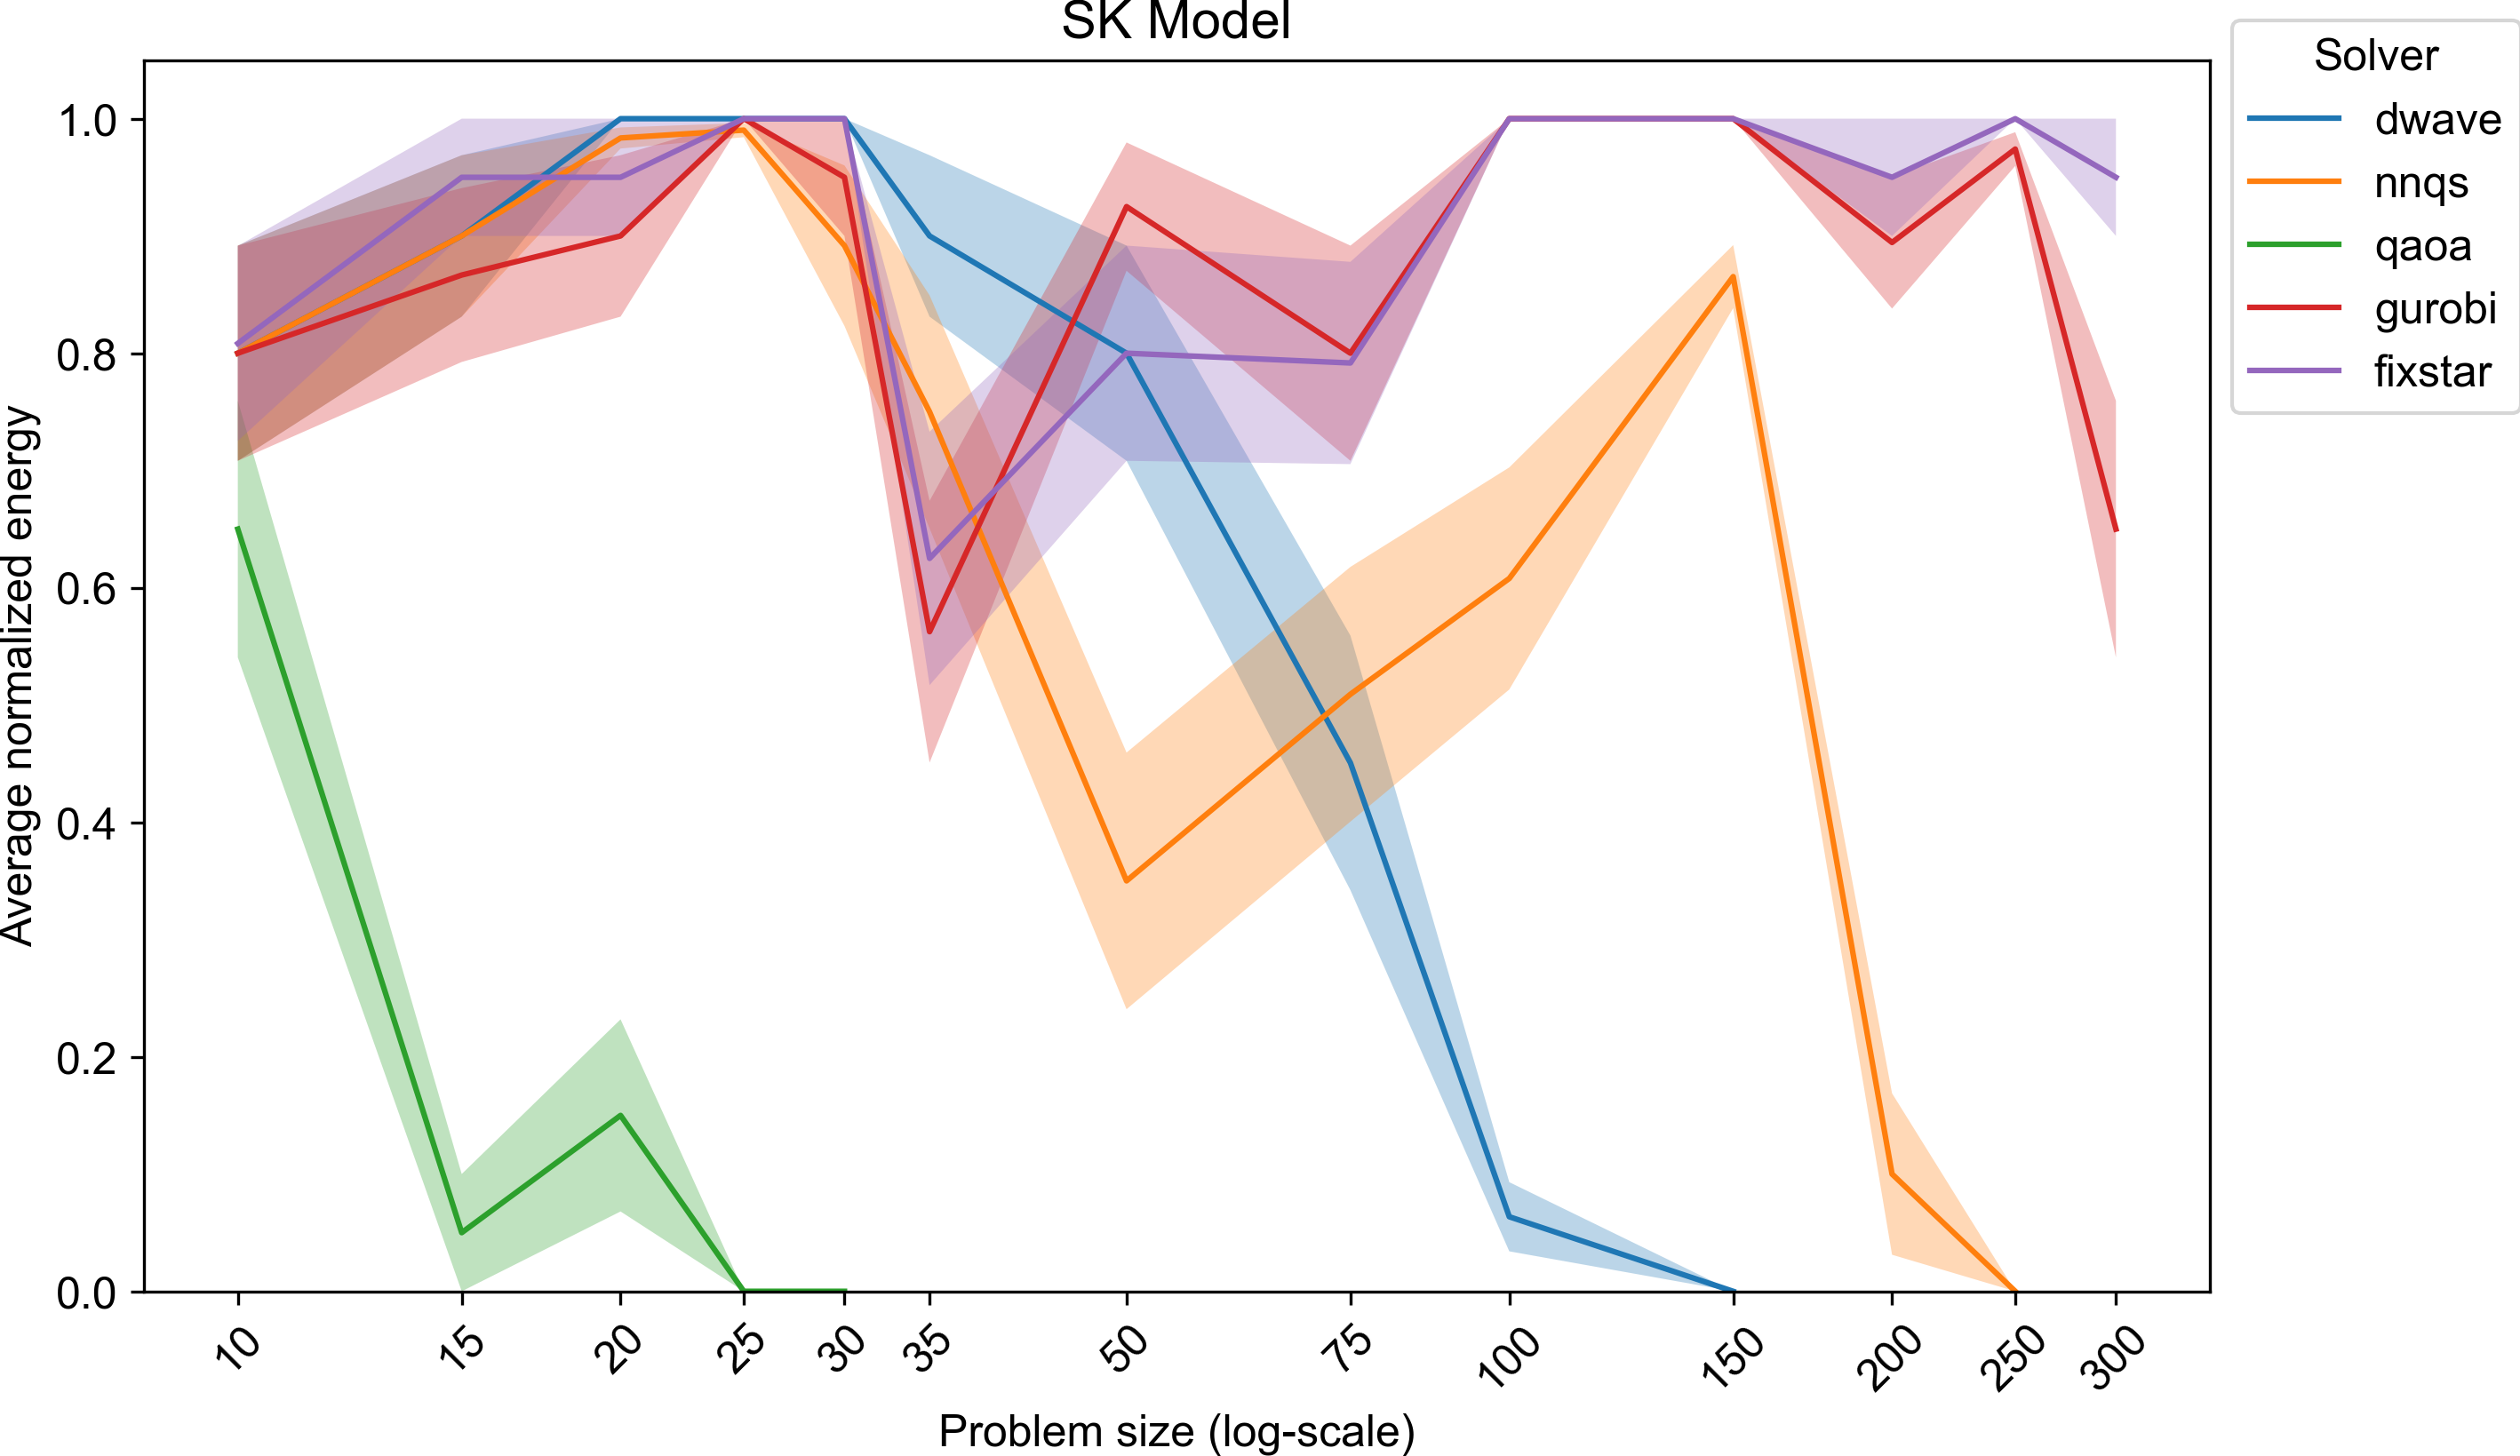
\includegraphics[width=0.9\textwidth]{images/skmodel_all_size.png}}%\hfill
    \\
    \subfloat[Success probability]{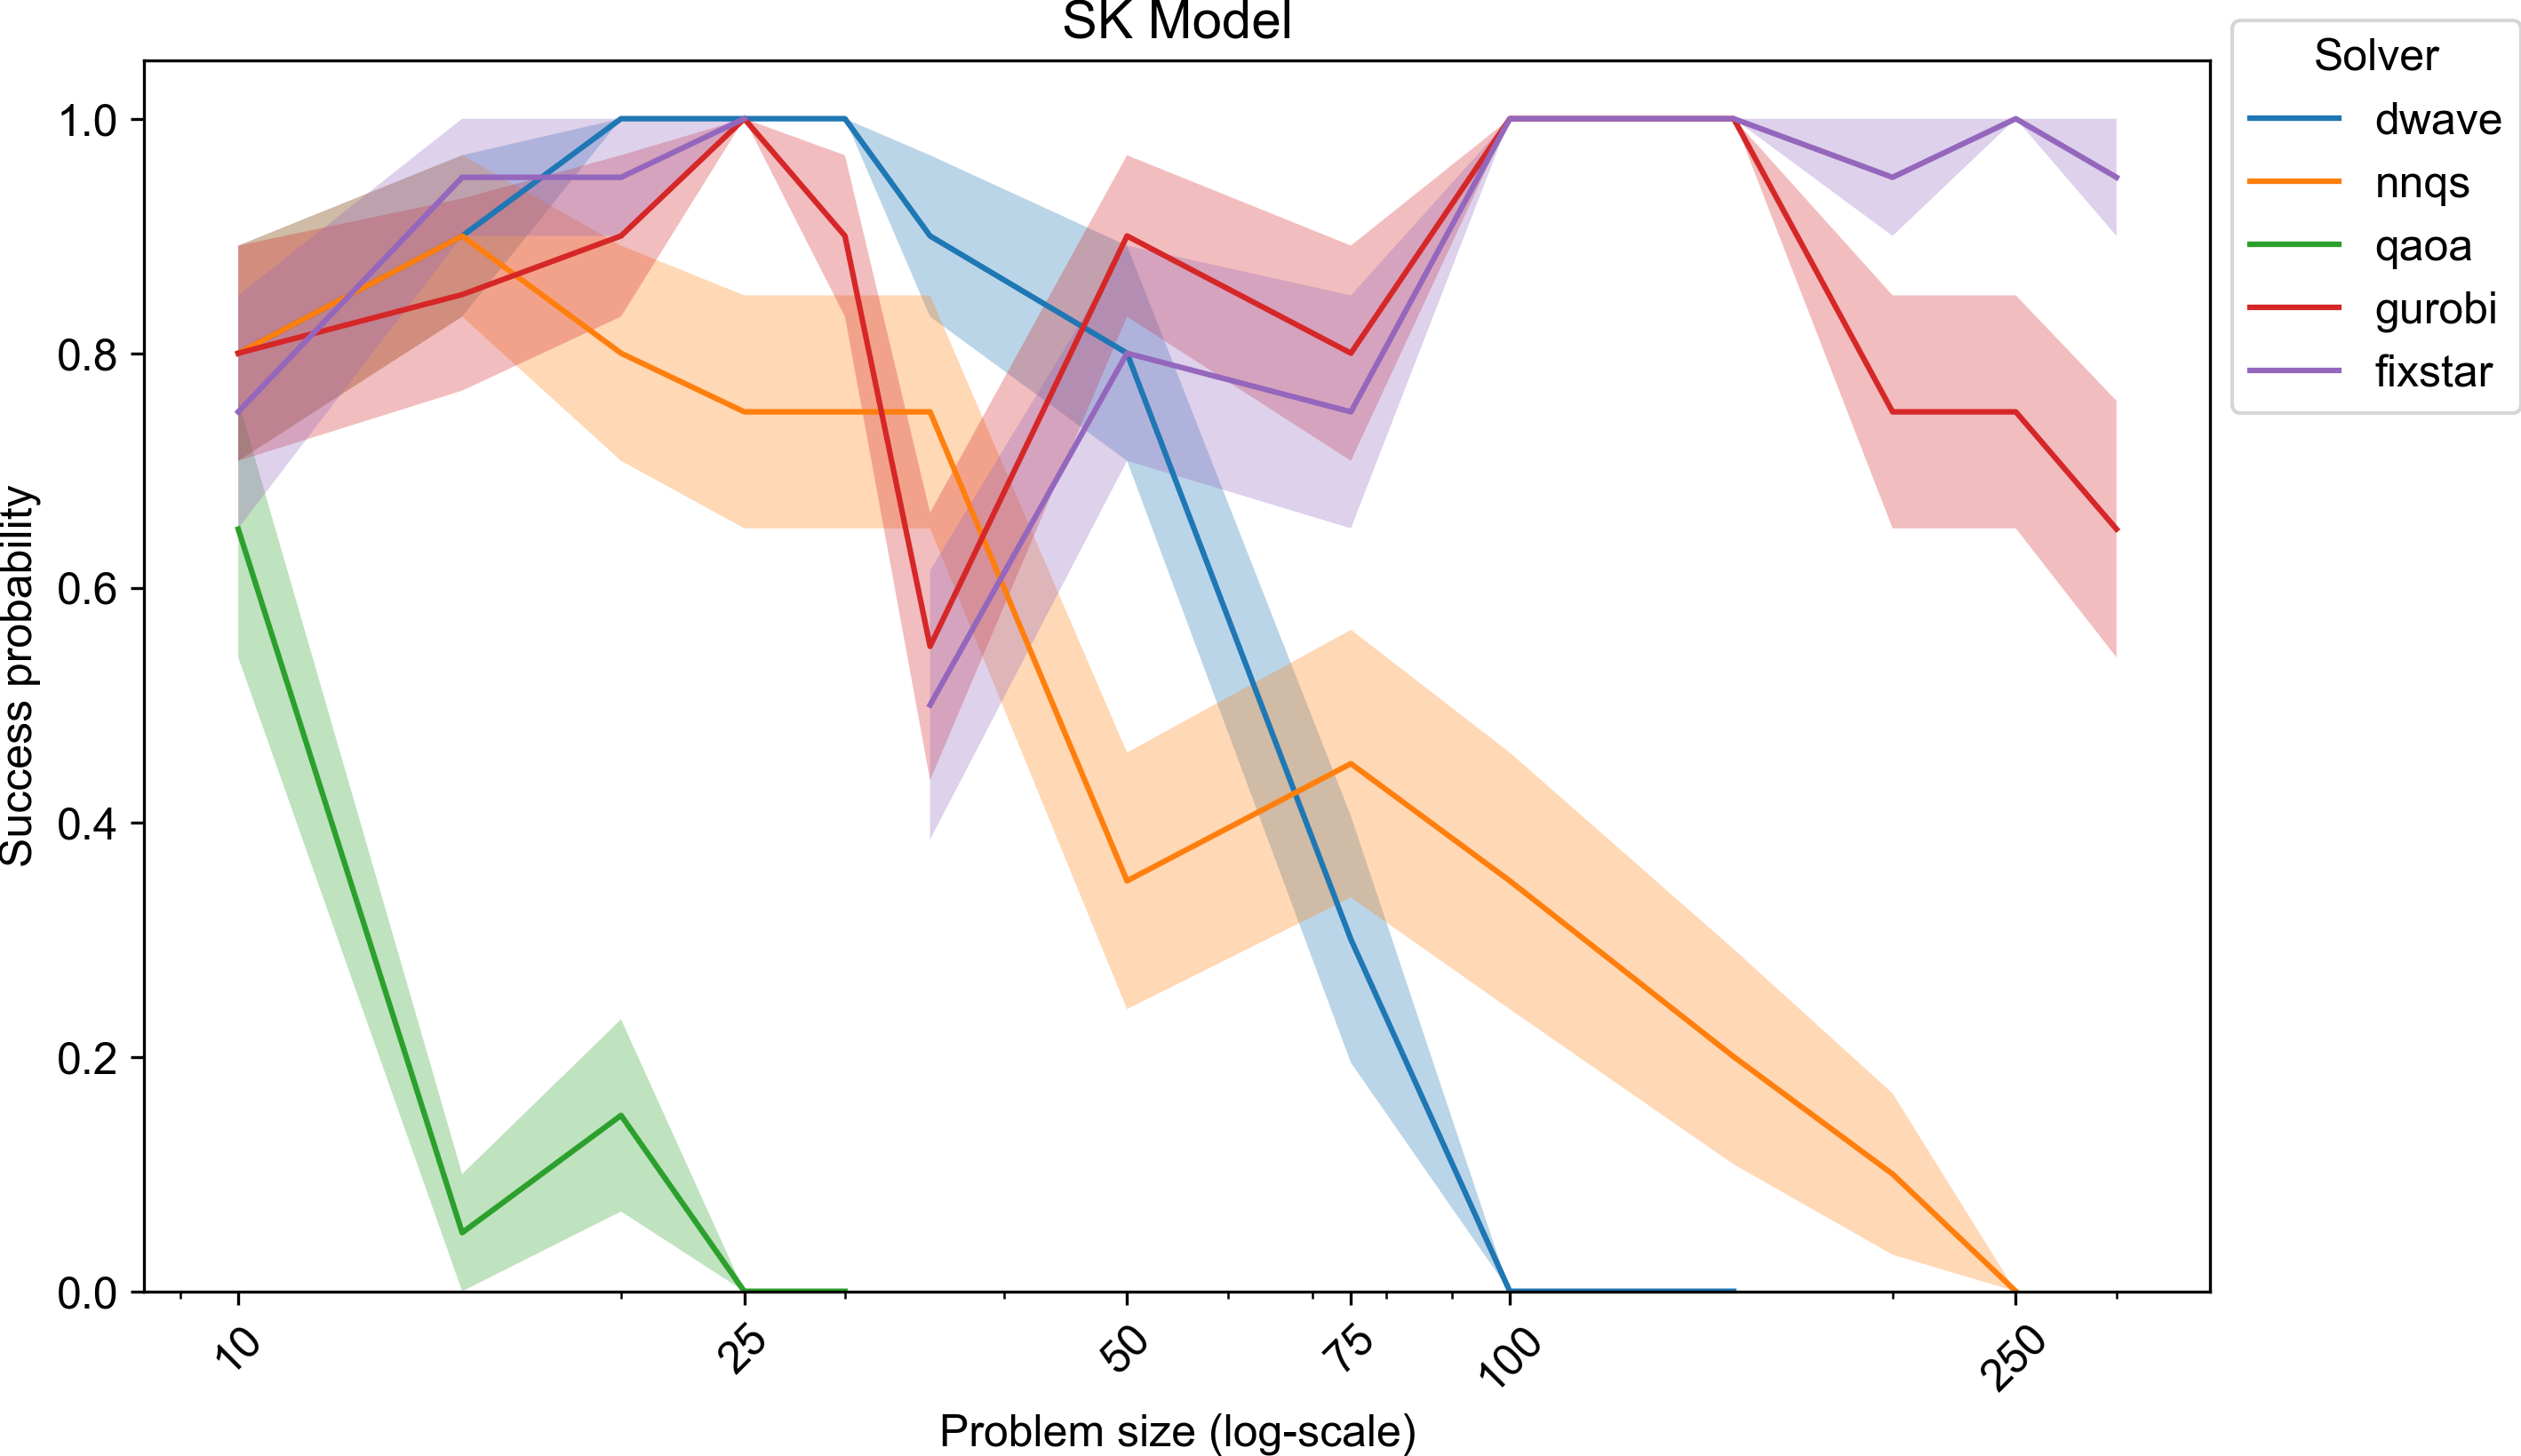
\includegraphics[width=0.9\textwidth]{images/skmodel_all_success_size.png}}
    \caption{Performance of different solvers for SK model by problem size}
    \label{all-skmodel-size}
\end{figure}

\begin{figure}[!htbp]
    \centering
    \subfloat[Normalized energy]{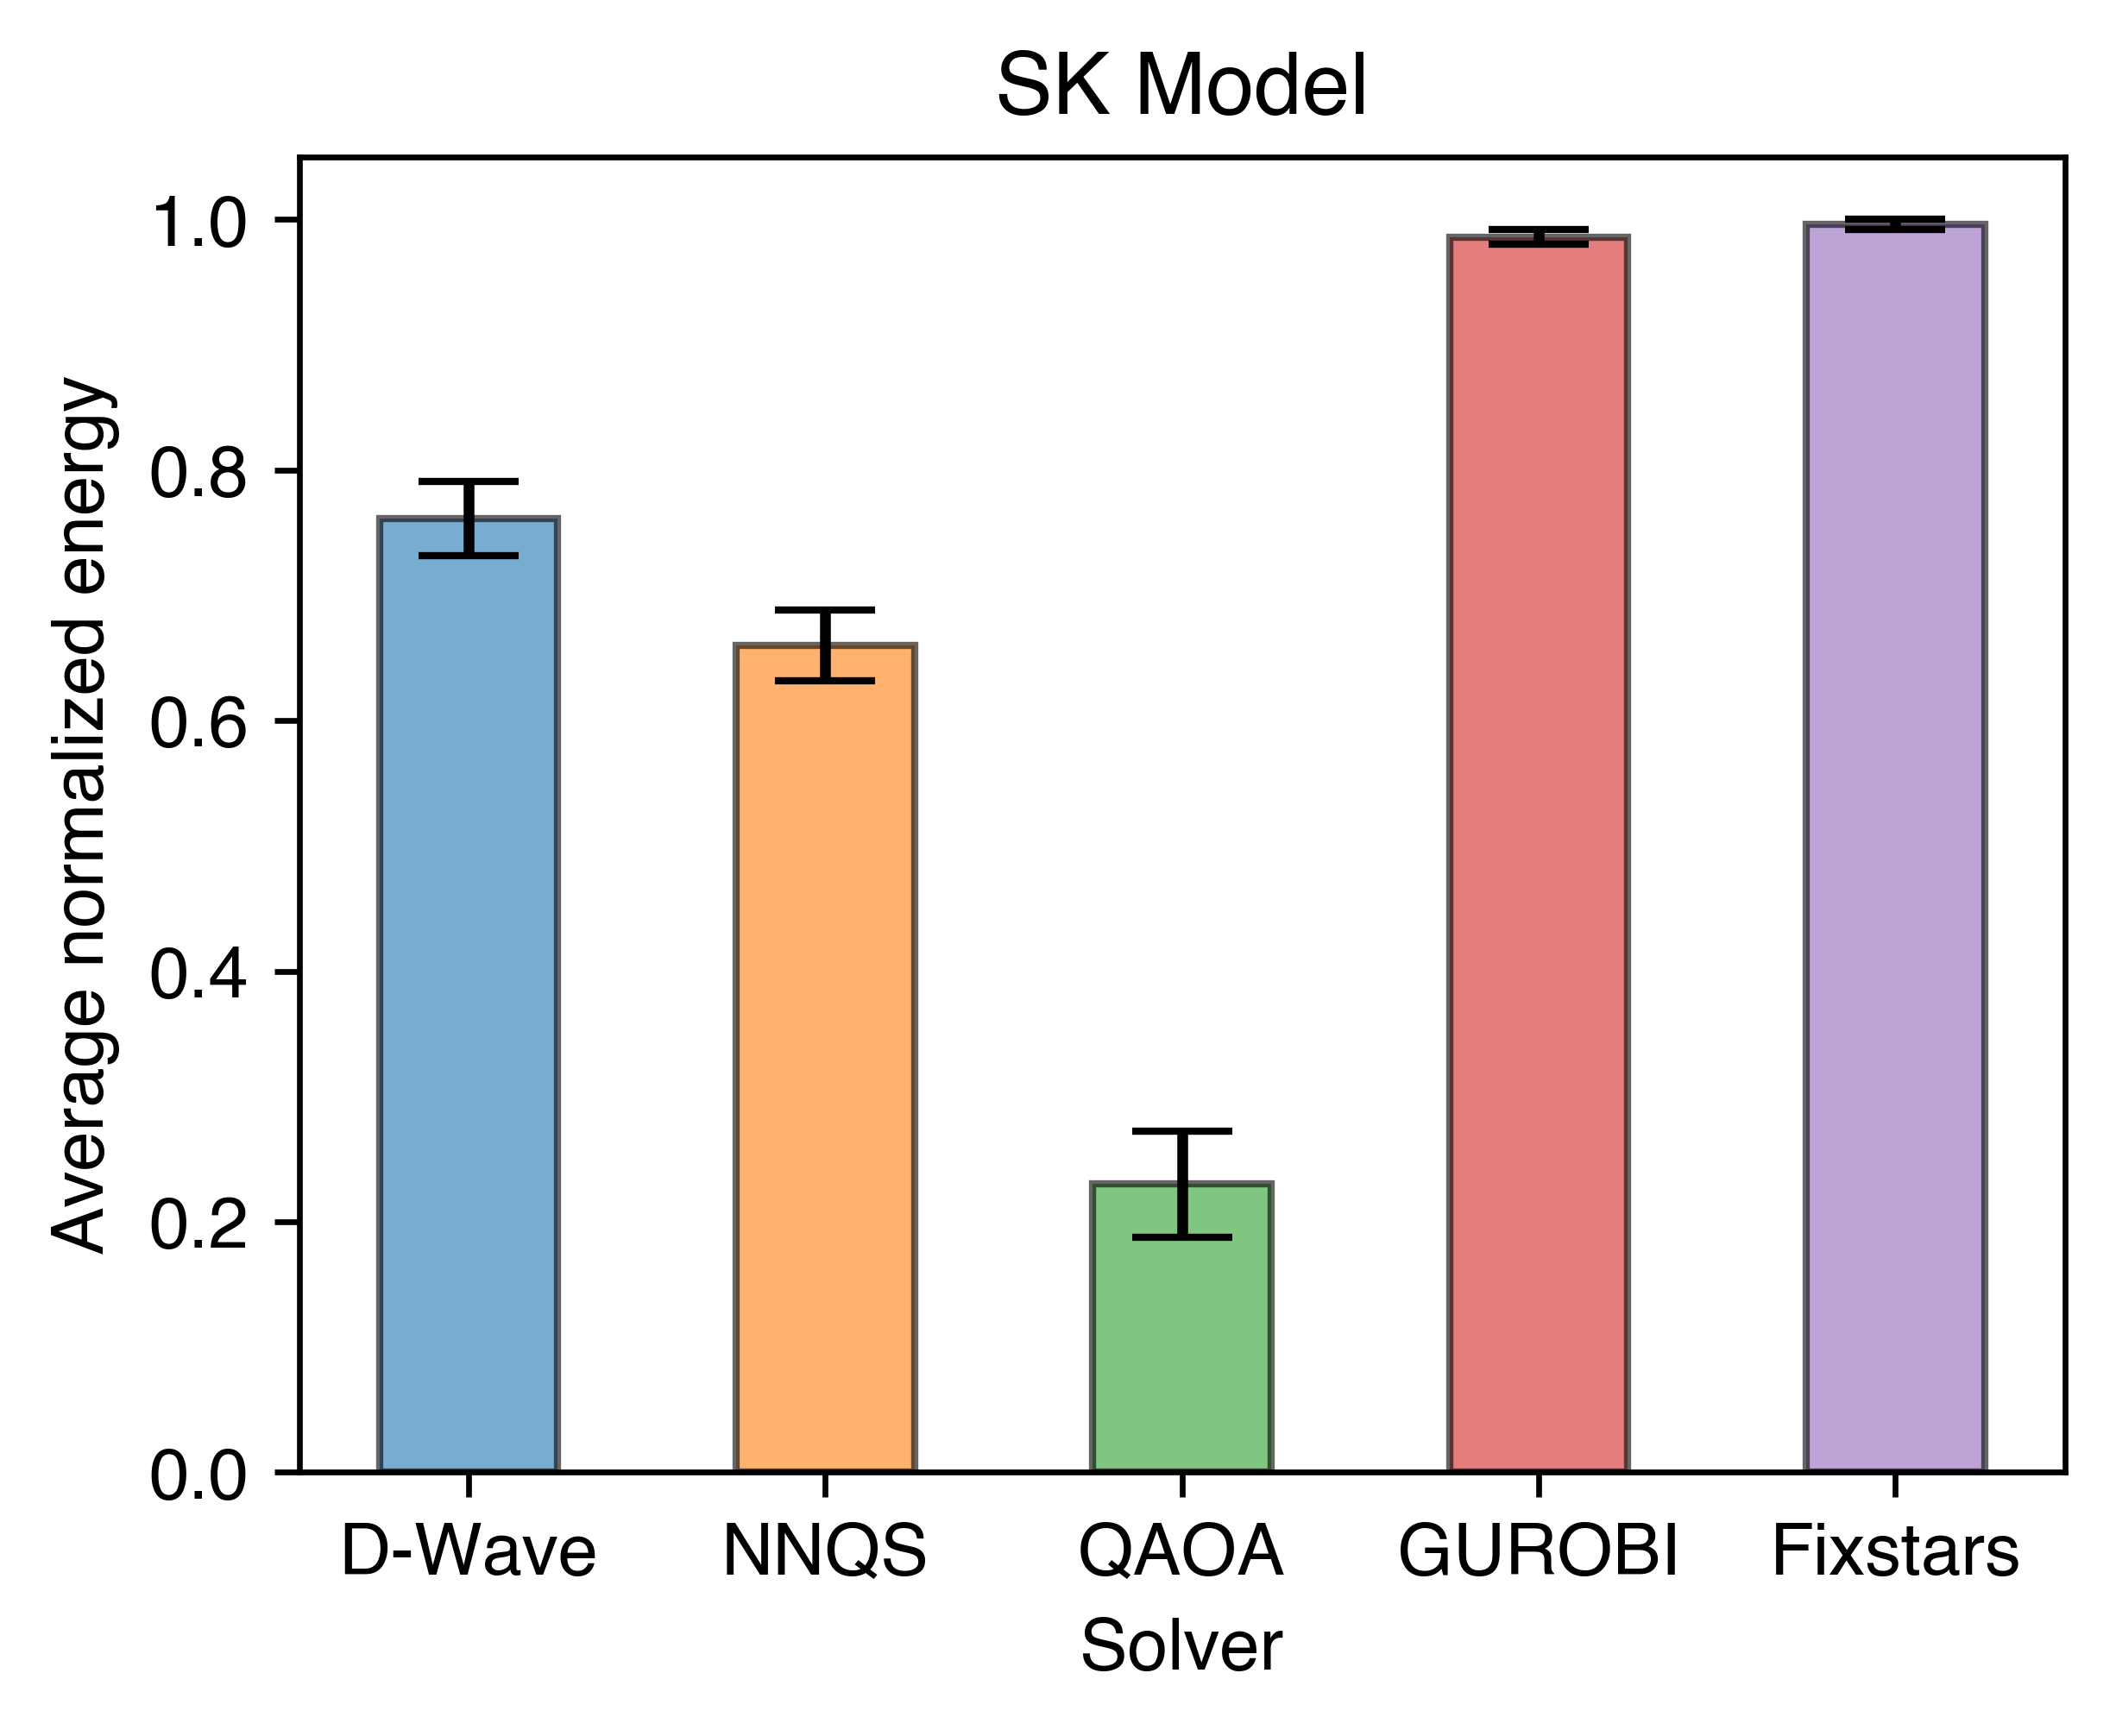
\includegraphics[width=0.49\textwidth]{images/skmodel_all_avg.png}}\hfill
    \subfloat[Success probability]{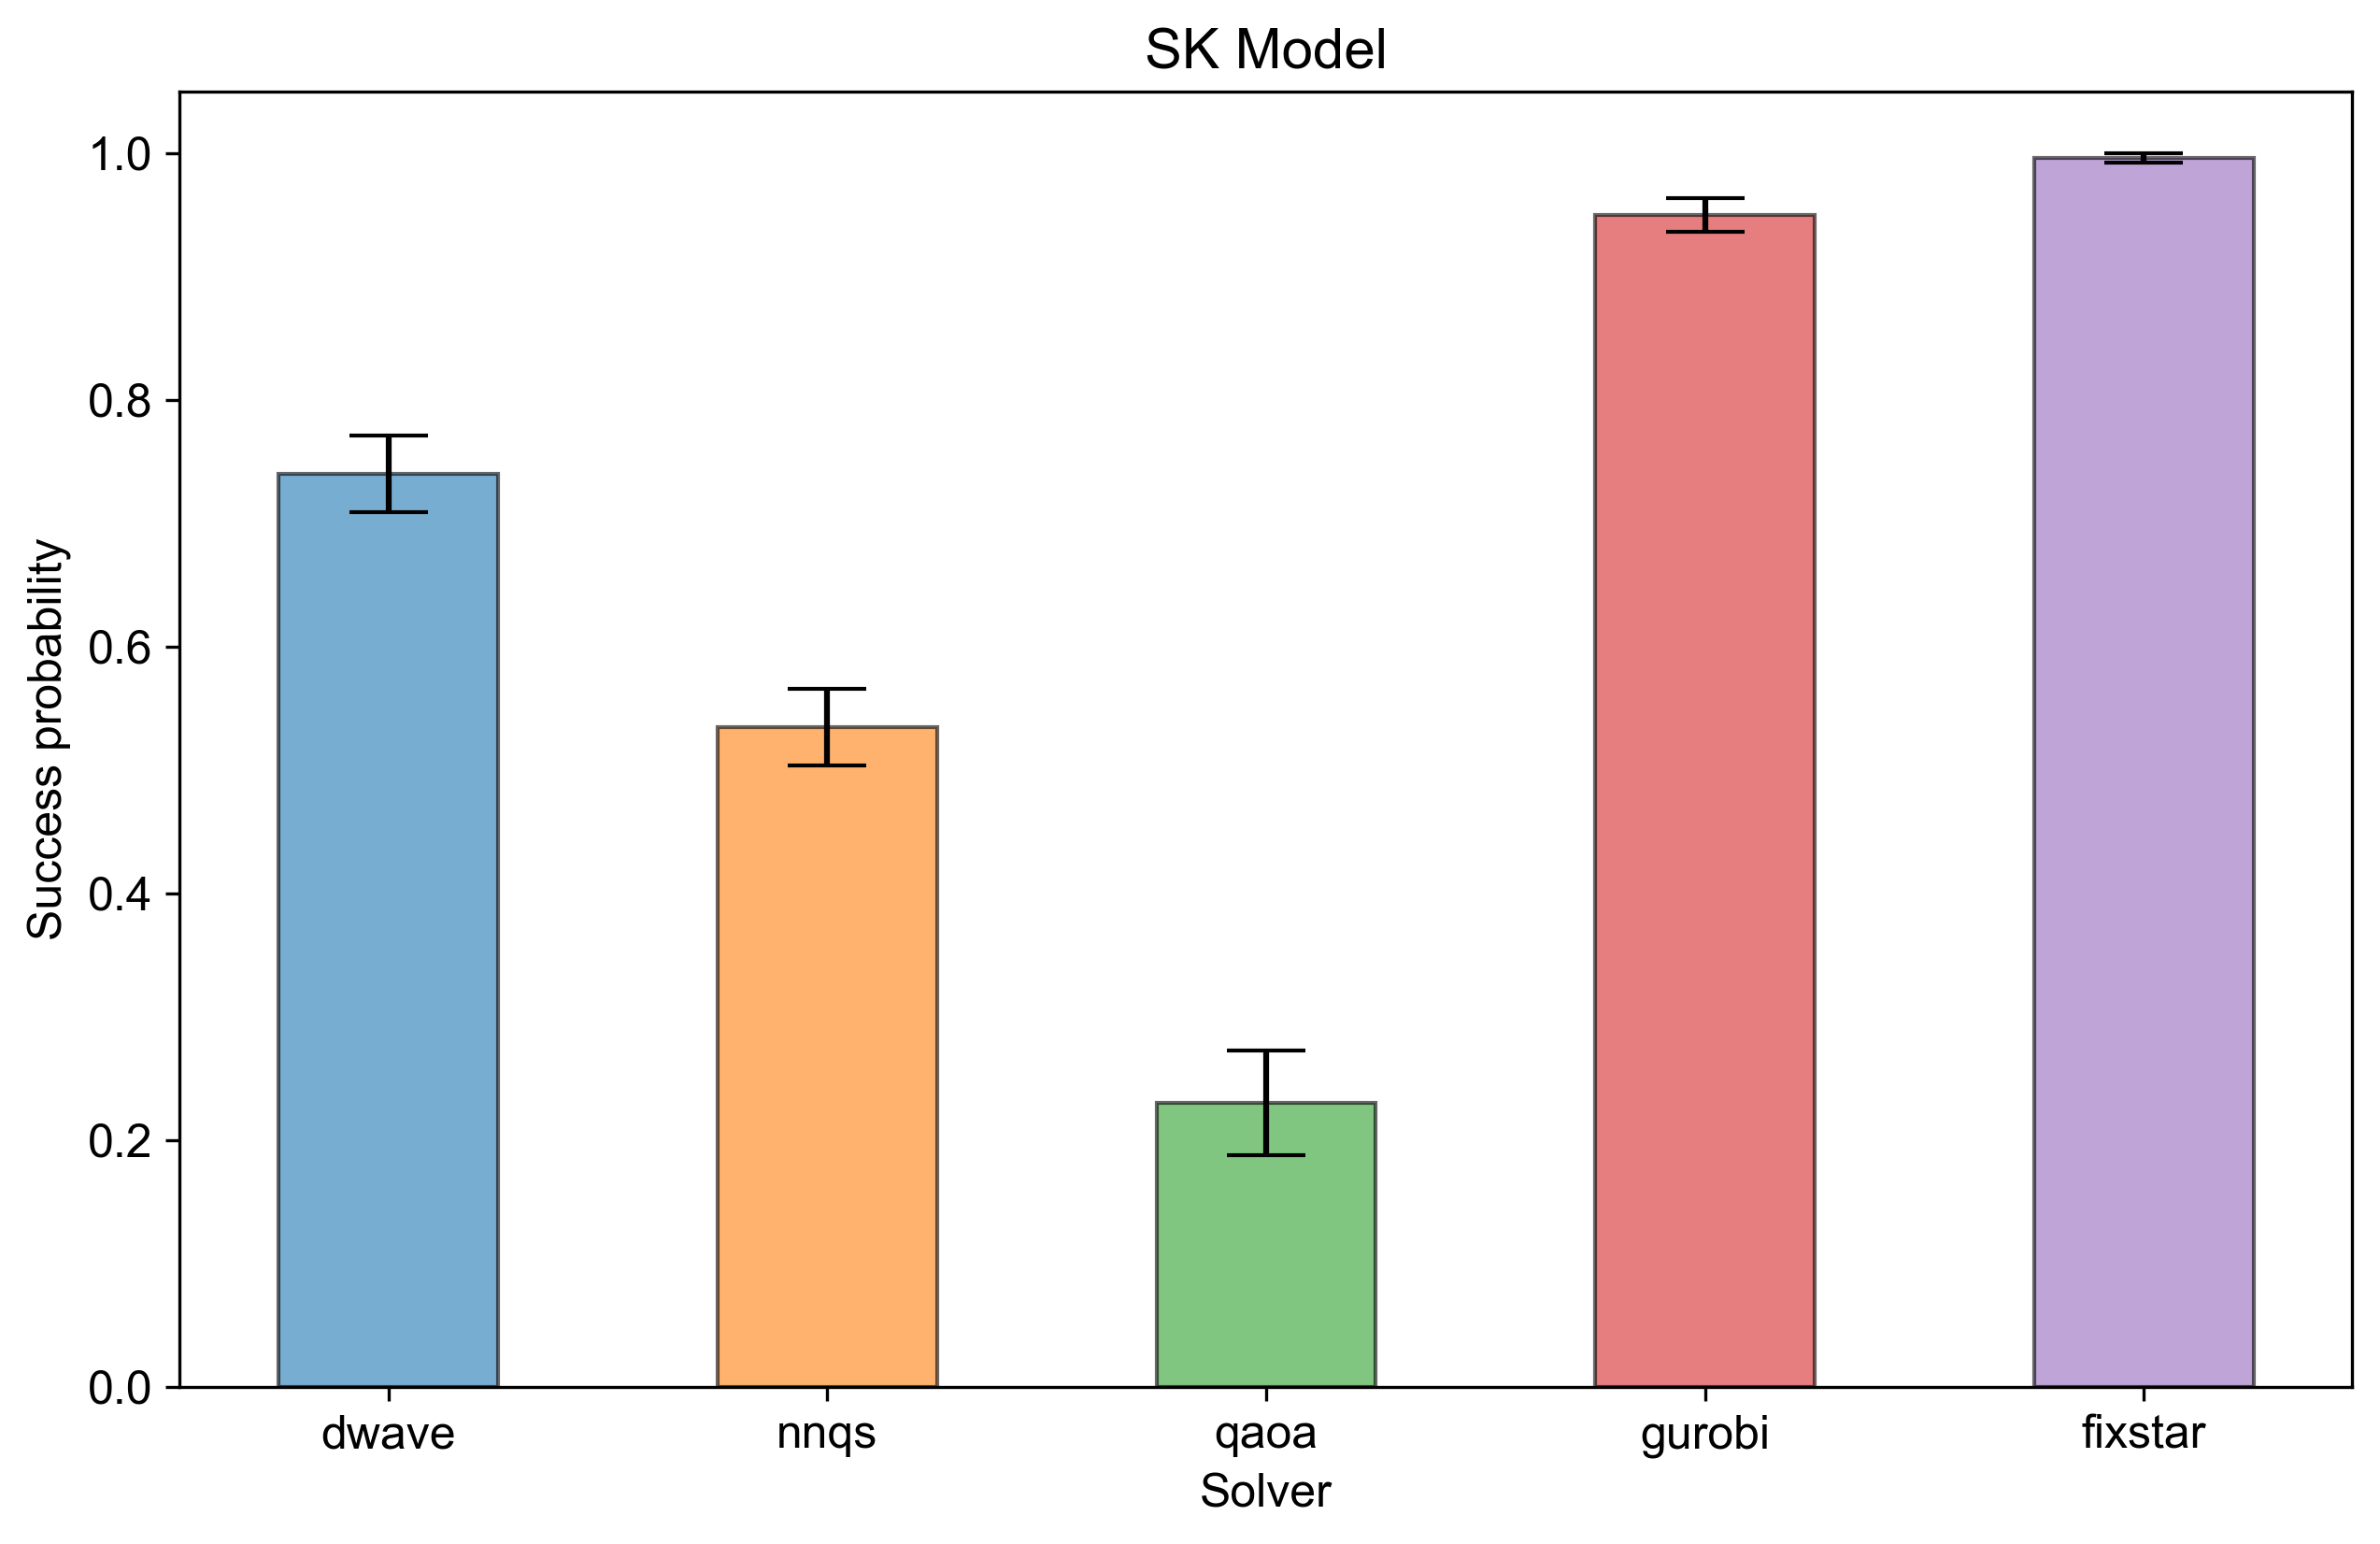
\includegraphics[width=0.49\textwidth]{images/skmodel_all_success_avg.png}}
    \caption{Average performance of different solvers for SK model}
    \label{all-skmodel-average}
\end{figure}

Performance by size for the SK model dataset is shown in \autoref{all-skmodel-size}, and average performance is shown in \autoref{all-skmodel-average}. For the SK model, the D-wave solver could only handle problem sizes up to $n=150$ due to the need for minor embedding onto the pegasus topology. The SK model is fully connected, which makes embedding difficult for the D-wave QPU. QAOA solved problems of up to $n=30$ due to the limitations of the simulator.

Due to its multi-valley energy landscape, the SK model presents a difficult problem for all QUBO solvers. The D-wave solver performs well up to $n=30$, gradually decreasing performance for larger problems. The NNQS follows a similar trend, although it can solve problems of larger sizes and performs better at sizes of $=100,150$. The QAOA solver has consistently poor performance across problem sizes.

Overall, the D-wave annealer has the highest average normalised energy and success probability among the three quantum-inspired solvers. The NNQS is slightly worse in both metrics, while the QAOA solver performs poorly for both metrics.

\section{Time-Constrained Solver Comparison}
We also measured the runtime for each solver for each problem and the average runtime across all problems with the same size $n$ shown in \autoref{results:timeaverage}. Runtimes split by problem type can be found in \autoref{appendix:timesizegraph}

For the D-wave solver, the average runtime increases approximately linearly from $0.128\si{\second}$ for $n=10$ to $0.184\si{\second}$ for $n=50$ and $0.292\si{\second}$ for $n=300$. 

For the NNQS solver, the runtime does not increase significantly from $n=10$ to $n=150$ and remains around from $250\si{\second}$ to $350\si{\second}$ but increases sharply for larger $n \geq 200$ which could be due to memory issues with the GPU or the sampling may have taken a longer time to converge. 

The QAOA solver's runtime remains stable from $n=10$ to $n=20$ at around $38 \si{\second}$. However, it increases rapidly to $6847 \si{\second}$ at $n=30$ due to the need for more optimisation iterations and greater computational resources for the simulation.

The GUROBI optimiser was set with a maximum time limit of $600 \si{\second}$ but could finish solving before the time limit for most problems with $n \leq 35$. The Fixstar solver was configured with a maximum time limit of $100 \si{\second}$, the maximum possible duration, and each solve utilised the entire time limit.

\begin{figure}[!htbp]
    \centering
    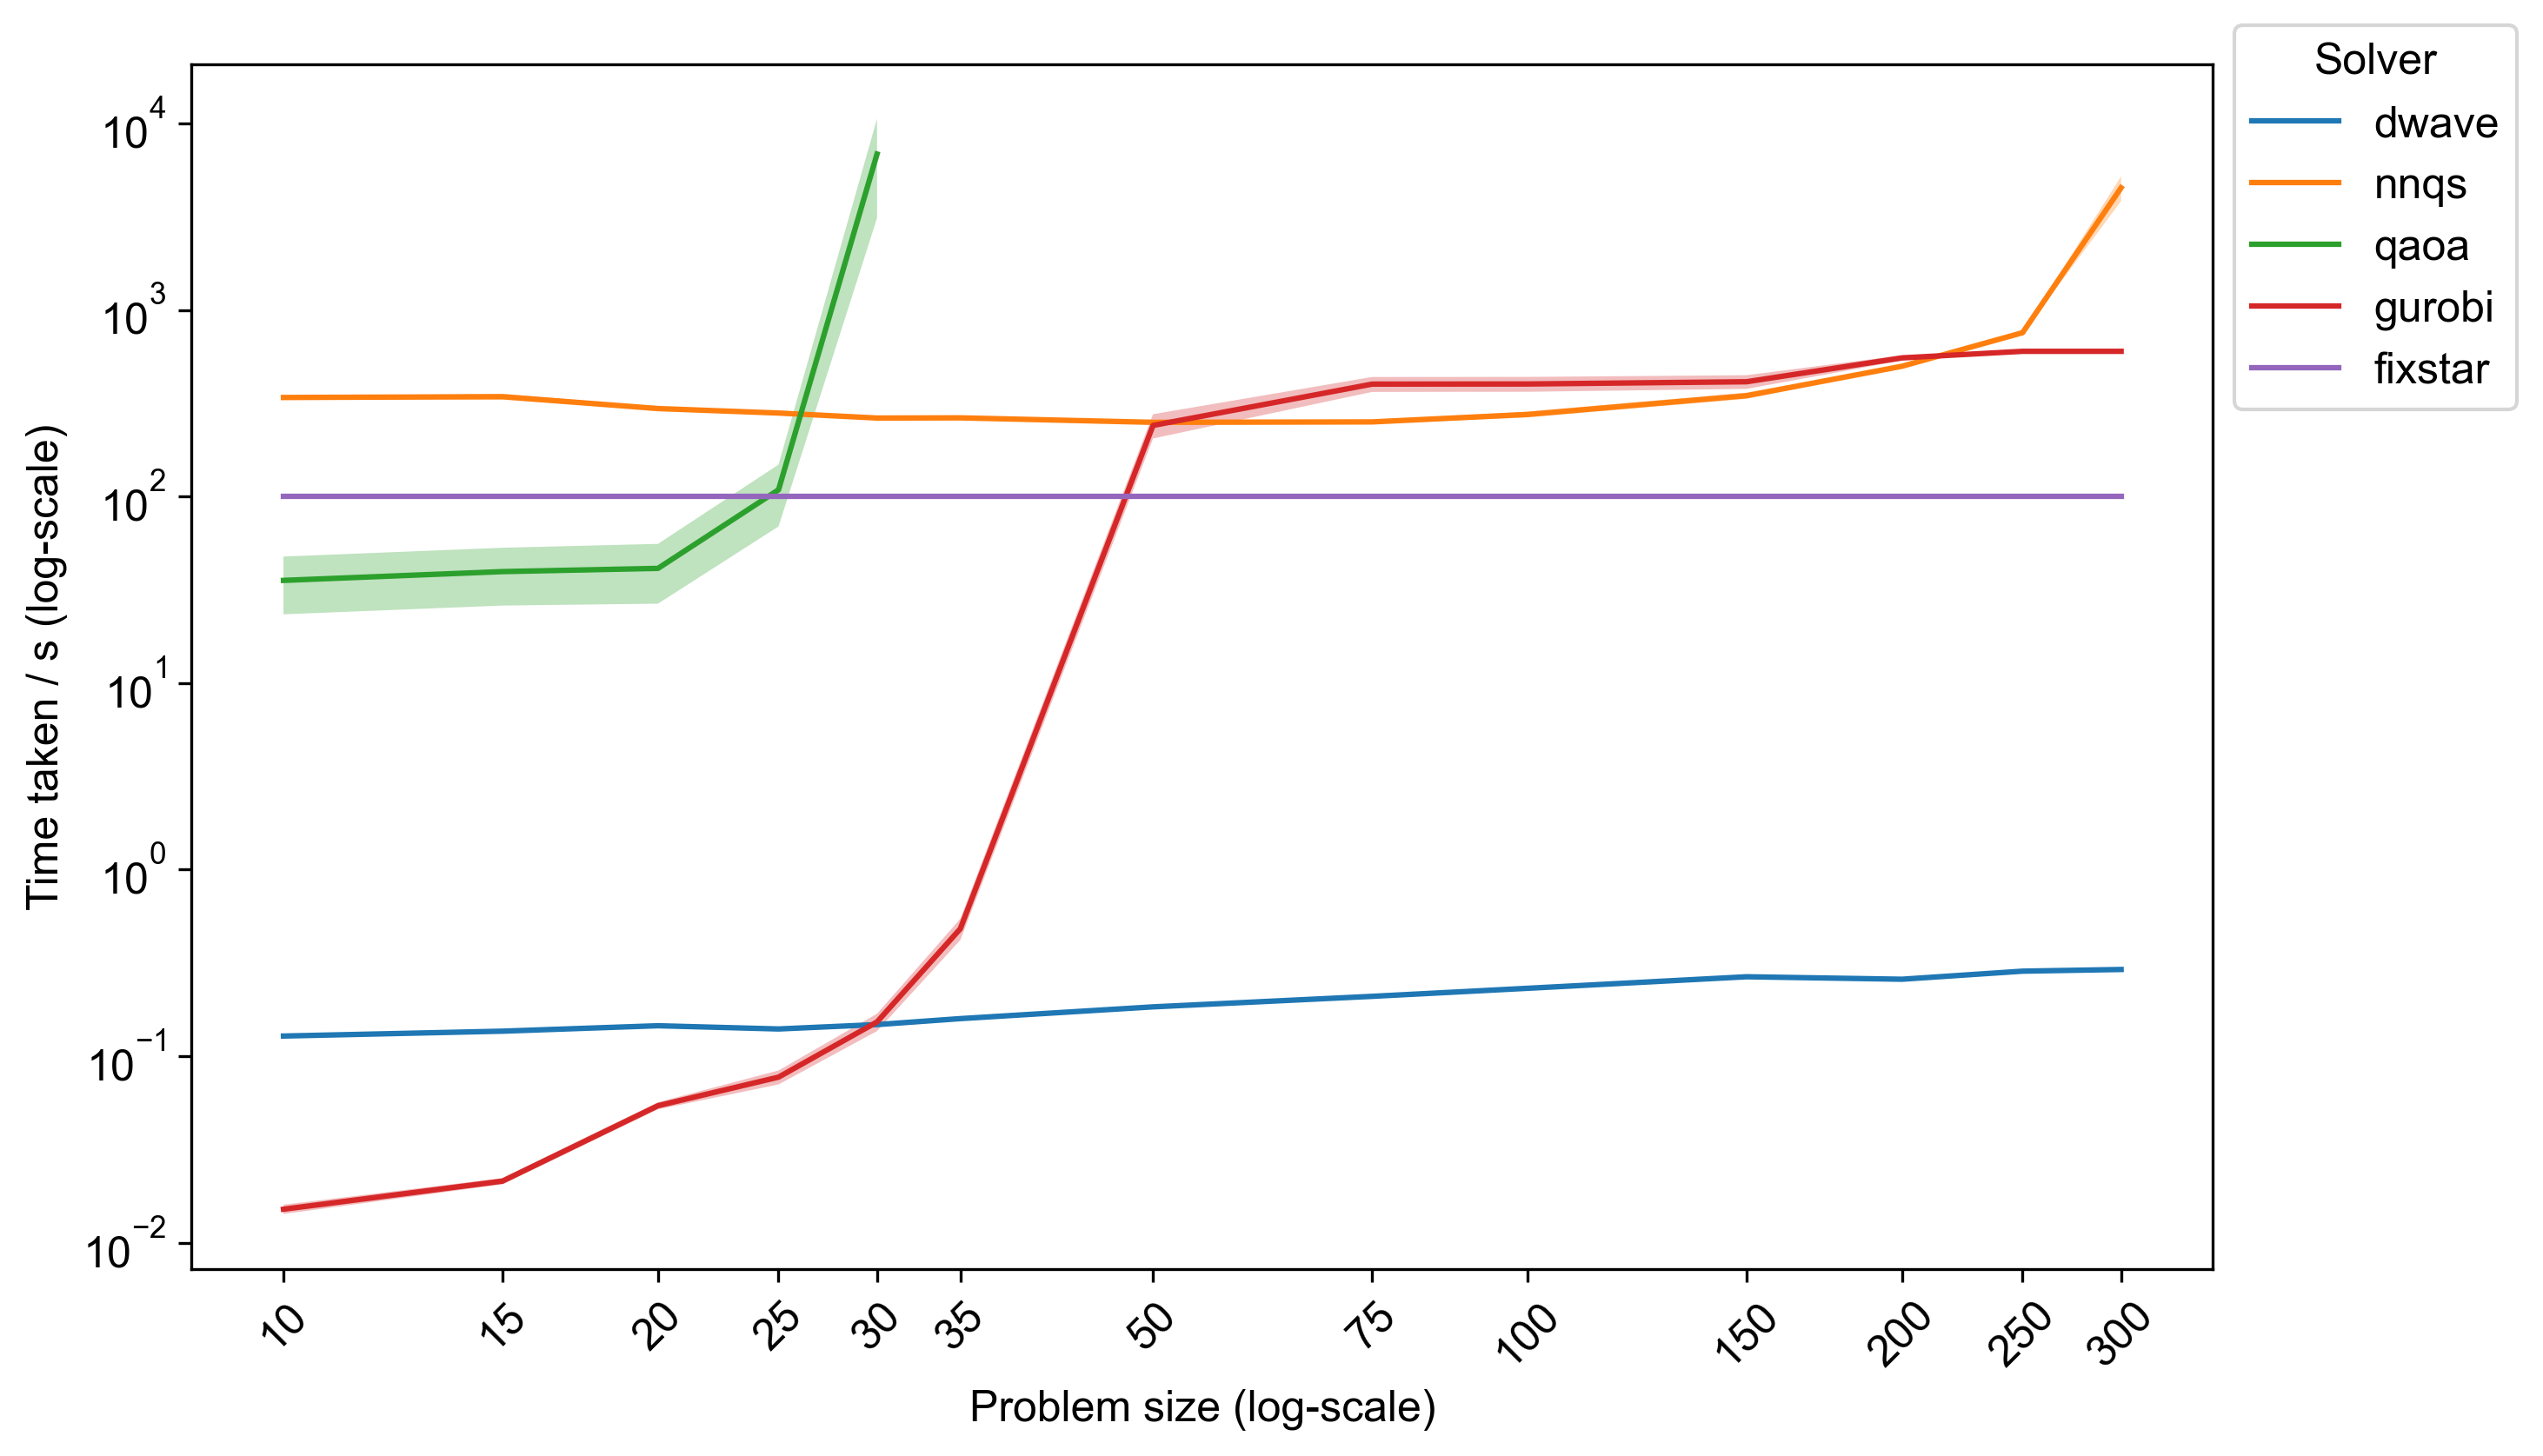
\includegraphics[width=0.9\textwidth]{images/all_time_average.png}
    \caption{Average runtime in log scale taken by different solvers for QUBO problems by size}
    \label{results:timeaverage}
\end{figure}

Using the average runtime of the D-wave solver, we conducted a second run of the benchmarking to measure the performance of the D-wave solver against the classical solvers---GUROBI and Fixstar. This experiment aimed to test if the D-wave solver could outperform the classical solvers if they were limited to the same runtime. For a problem of a specific type and size, the classical solvers were run with a maximum runtime equal to the average time required by the D-wave solver for problems of equivalent type and size shown in \autoref{results:averageruntimedwave}.

\begin{table}[!ht]
    \centering
    \resizebox{\textwidth}{!}{%
    \begin{tabular}{lrrrrrrrrrrrrr} \toprule
        $n$ & 10 & 15 & 20 & 25 & 30 & 35 & 50 & 75 & 100 & 150 & 200 & 250 & 300 \\ \midrule
        NAE3SAT & 0.133 & 0.135 & 0.141 & 0.149 & 0.138 & 0.156 & 0.173 & 0.184 & 0.201 & 0.243 & 0.259 & 0.286 & 0.292 \\
        Max-cut & 0.127 & 0.136 & 0.1560 & 0.130 & 0.155 & 0.160 & 0.183 & 0.223 & 0.247 & 0.278 & - & - & - \\
        SK model & 0.125 & 0.137 & 0.140 & 0.140 & 0.150 & 0.161 & 0.195 & 0.221 & 0.245 & 0.278 & - & - & - \\ \bottomrule
    \end{tabular}}
    \caption{Average runtime (seconds) of the D-wave solver by problem type and size. Dashes indicate that the D-wave solver could not embed problems of that size.}
    \label{results:averageruntimedwave}
\end{table}

The results are shown in \autoref{all-time-size}. For each problem type, the performance of the GUROBI solver drops before the D-wave solver, and there are problem types and sizes where the D-wave solver outperforms the GUROBI solver when the runtime is matched. The D-wave solver outperforms GUROBI for NAE3SAT with $n=50, 75$, max-cut with $n=30,35$, and SK model with $n=20, 35$. However, when the problem sizes increase even further, the D-wave solver performs poorly, possibly due to the increased noise of the quantum annealer. The Fixstar solver remains the top-performing solver across all problem types and sizes, even when the runtime is matched with the D-wave solver. The results show that the D-wave solver can outperform classical solvers like GUROBI for specific problem sizes when the runtime is matched.

\begin{figure}[!htbp]
    \centering
    \subfloat[NAE3SAT]{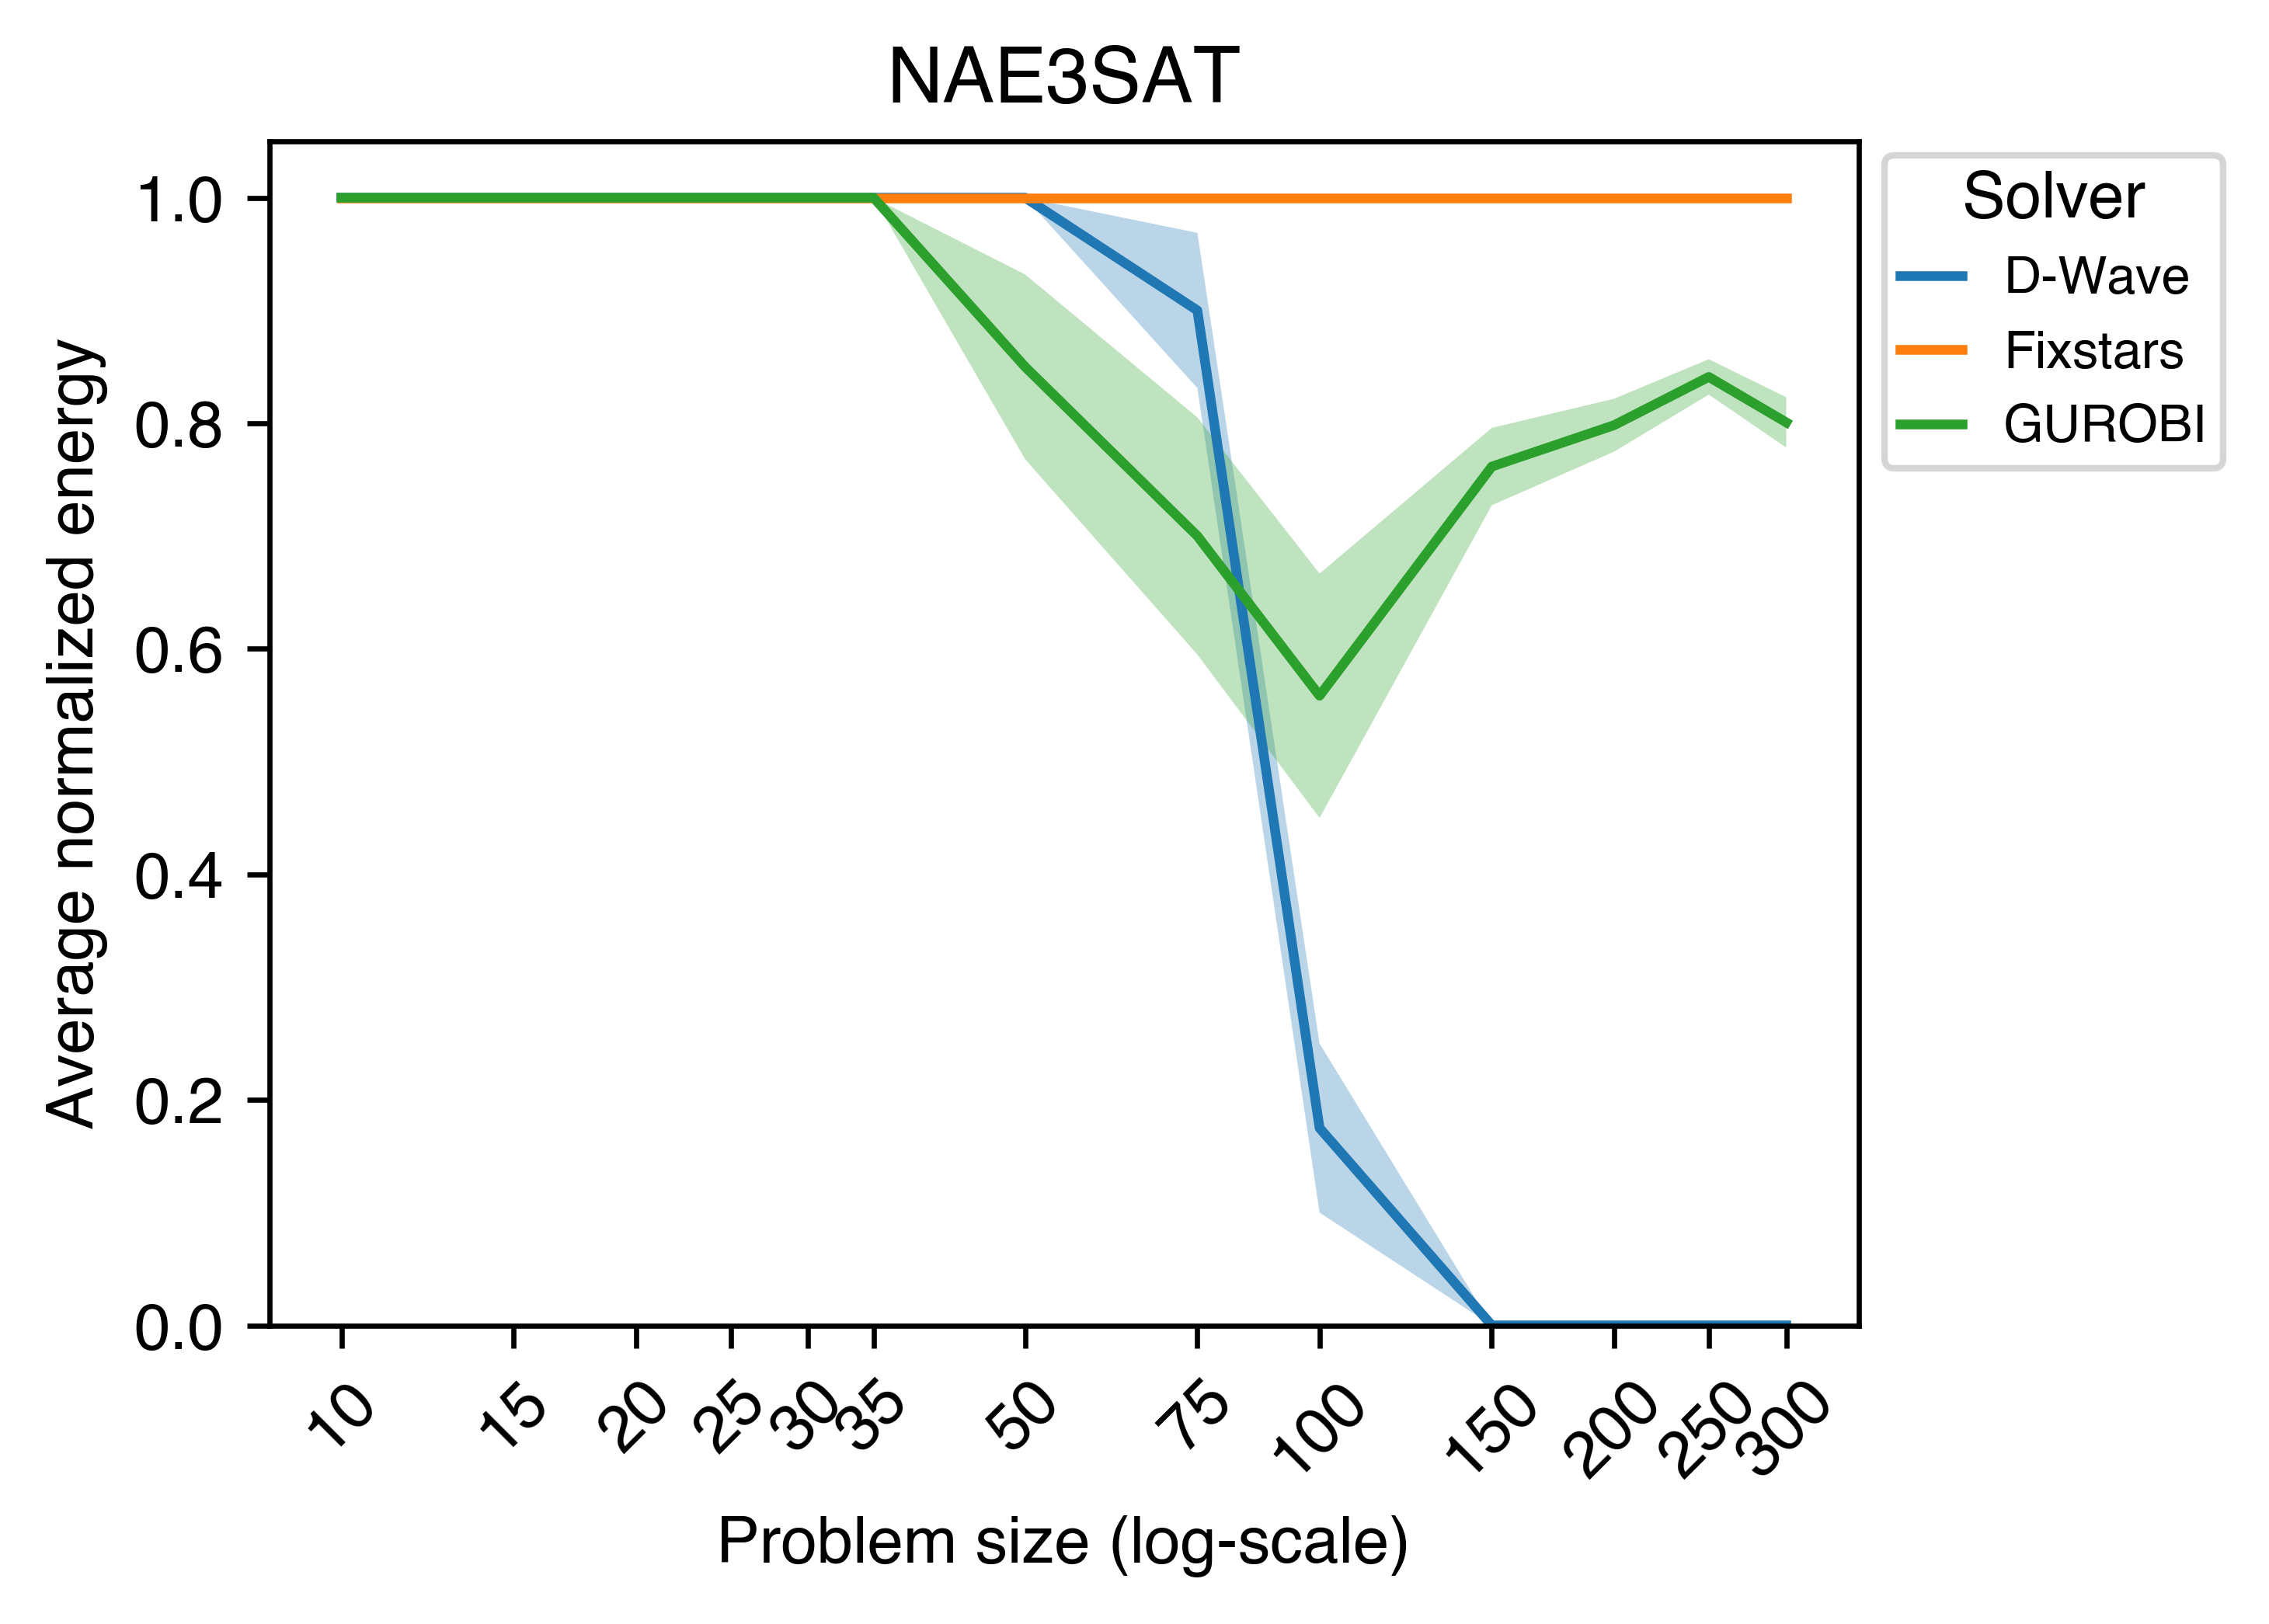
\includegraphics[width=0.7\textwidth]{images/nae3sat_timing_size.png}}%\hfill
    \\
    \subfloat[Max-cut]{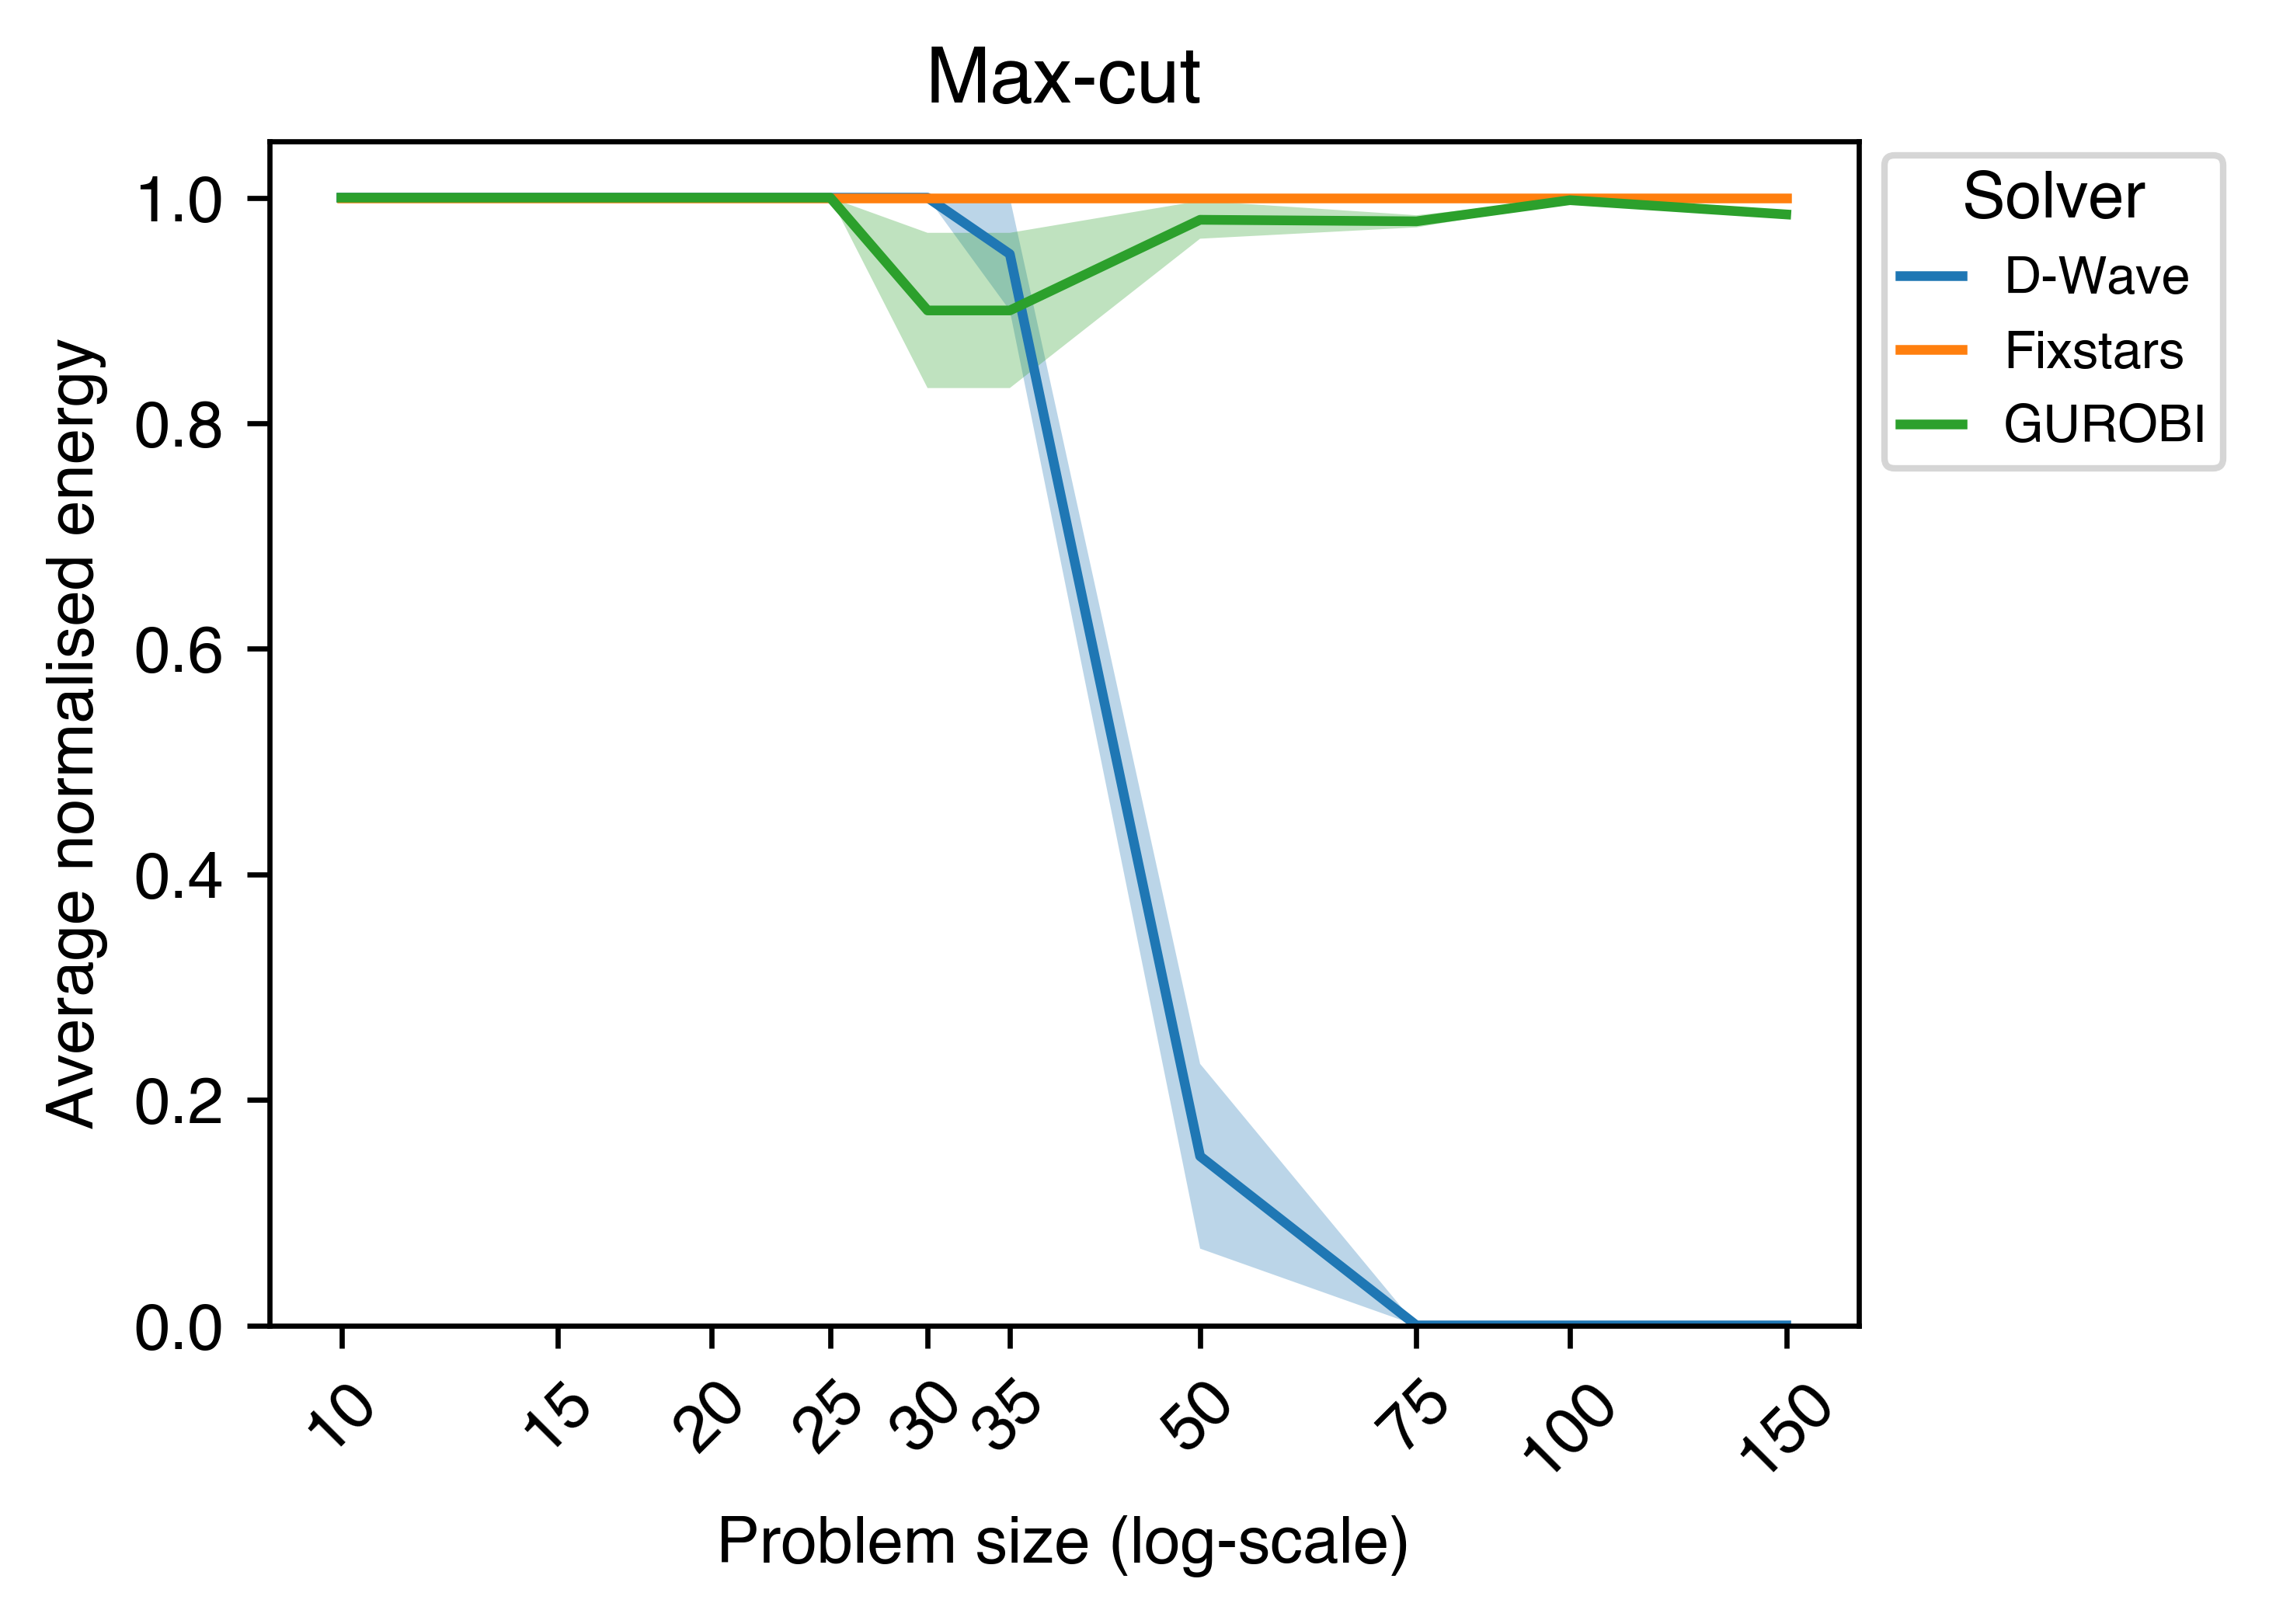
\includegraphics[width=0.7\textwidth]{images/maxcut_timing_size.png}}
    \\    
    \subfloat[SK model]{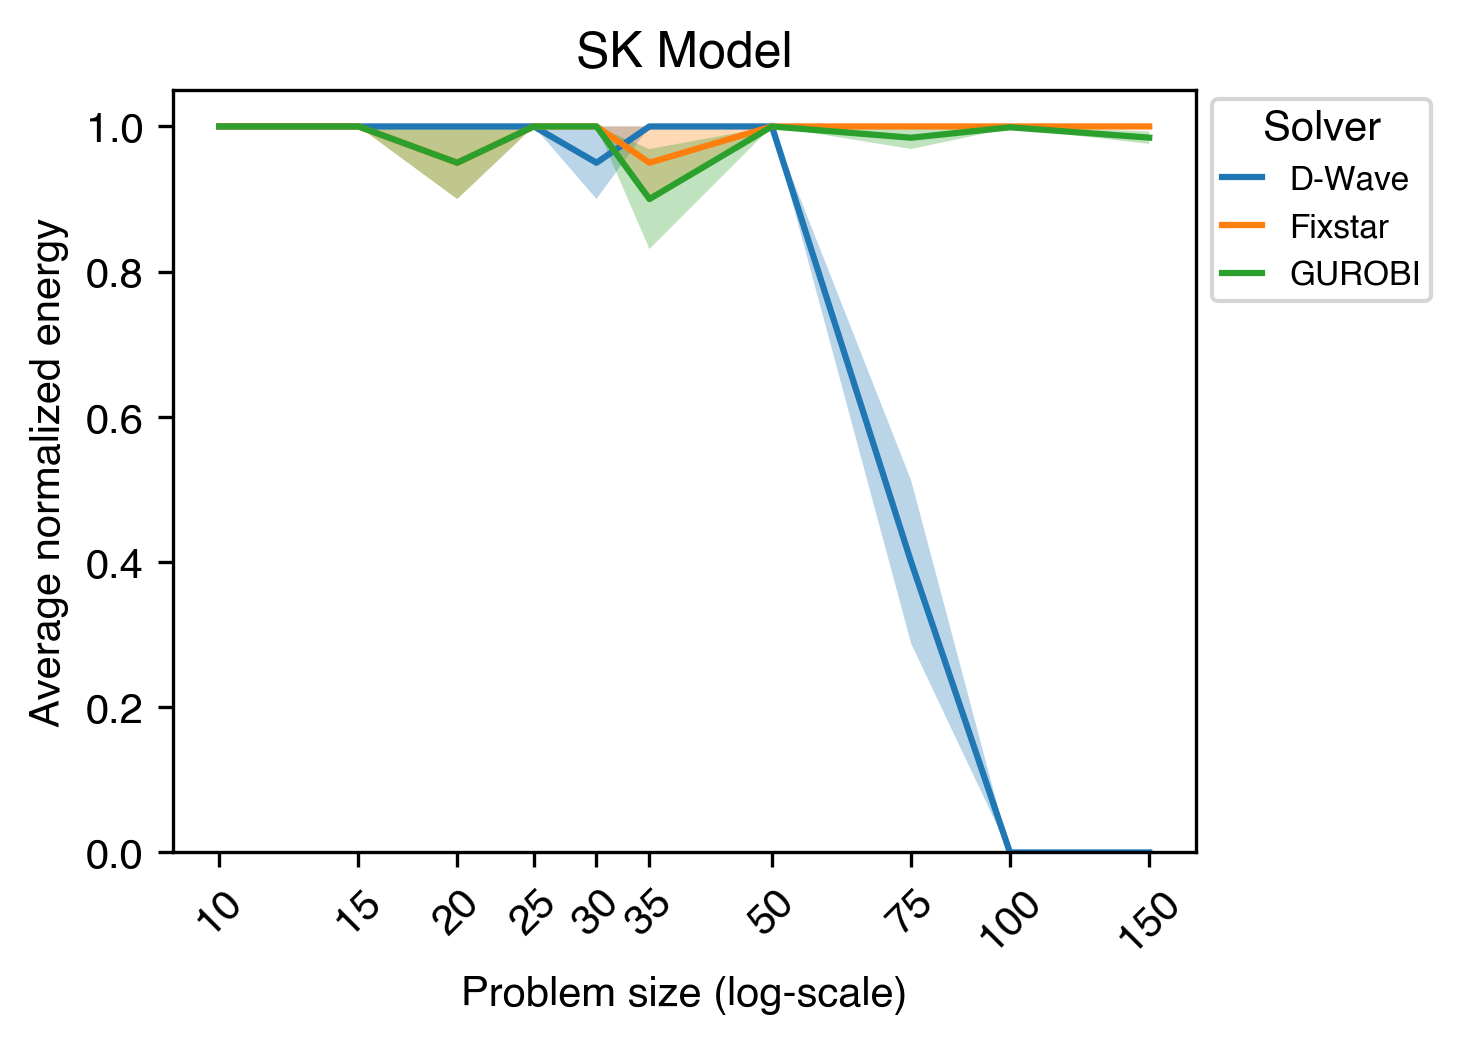
\includegraphics[width=0.7\textwidth]{images/skmodel_timing_size.png}}
    \caption{Performance of D-wave solver against GUROBI and Fixstar by problem type and size}
    \label{all-time-size}
\end{figure}

\section{Solver logs}
During the benchmarking experiments, supplementary metadata from the D-wave and QAOA solver was recorded. We recorded the embedded qubit count for the D-wave solver, which tends to grow differently for different problem types. For the QAOA solver, we recorded the number of quantum gates and the circuit depth, which can help quantify the complexity of the quantum circuit used. A metadata summary is available in \autoref{appendix:metadata}.

\section{Conclusion}
When comparing the three quantum-inspired solvers, NNQS has the best normalised energy for the NAE3SAT and max-cut dataset, while the D-wave solver has the best normalised energy for the SK model performance. NNQS also does the best in normalised energy when averaged across the three datasets. NNQS tends to do better in normalised energy since it minimises the energy expectation value, which optimises the average energy of samples but does not necessarily optimise for the highest probability of sampling the best solution. 

QAOA has the highest success probability for the NAE3SAT dataset. However, it is important to note that it could only handle problems with up to $30$ variables. The D-wave solver has the best success probability for the max-cut and SK model datasets and the average success probability across the three datasets.

\autoref{results:allnormalizedenergy} and \autoref{results:allsuccess} show the average normalised energy and success probability for different solvers for each dataset and the average across all datasets. Across all datasets and both metrics, the Fixstar QUBO solver has the best performance, consistently returning the best solutions out of all solvers.


\begin{table}[!ht]
    \centering
    \begin{tabular}{cccccc} \toprule
        ~ & D-wave & NNQS & QAOA & GUROBI & Fixstar \\ \midrule
        NAE3SAT & 0.617 & \textbf{0.755} & 0.640 & 0.983 & 1.00 \\
        Max-cut & 0.610 & \textbf{0.753} & 0.190 & 0.991 & 1.00 \\
        SK model & \textbf{0.761} & 0.664 & 0.230 & 0.990 & 1.00 \\ \midrule
        Average & 0.663 & \textbf{0.724} & 0.353 & 0.988 & 1.00 \\ \bottomrule
    \end{tabular}
    \caption{Average normalised energy for different solvers}
    \label{results:allnormalizedenergy}
\end{table}

\begin{table}[!ht]
    \centering
    \begin{tabular}{cccccc} \toprule
        ~ & D-wave & NNQS & QAOA & GUROBI & Fixstar \\ \midrule
        NAE3SAT & 0.615 & 0.538 & \textbf{0.640} & 0.858 & 1.00 \\
        Max-cut & \textbf{0.610} & 0.585 & 0.190 & 0.931 & 1.00 \\
        SK model & \textbf{0.740} & 0.538 & 0.230 & 0.954 & 1.00 \\ \midrule
        Average & \textbf{0.655} & 0.554 & 0.353 & 0.914 & 1.00 \\ \bottomrule
    \end{tabular}
\caption{Success probability for different solvers}
\label{results:allsuccess}
\end{table}

